%% 
%% Copyright 2007-2020 Elsevier Ltd
%% 
%% This file is part of the 'Elsarticle Bundle'.
%% ---------------------------------------------
%% 
%% It may be distributed under the conditions of the LaTeX Project Public
%% License, either version 1.2 of this license or (at your option) any
%% later version.  The latest version of this license is in
%%    http://www.latex-project.org/lppl.txt
%% and version 1.2 or later is part of all distributions of LaTeX
%% version 1999/12/01 or later.
%% 
%% The list of all files belonging to the 'Elsarticle Bundle' is
%% given in the file `manifest.txt'.
%% 

%% Template article for Elsevier's document class `elsarticle'
%% with numbered style bibliographic references
%% SP 2008/03/01
%%
%% 
%%
%% $Id: elsarticle-template-num.tex 190 2020-11-23 11:12:32Z rishi $
%%
%%
%\documentclass[preprint,12pt]{elsarticle}
% \documentclass[review,12pt, 3p, times]{elsarticle}
\documentclass[review,12pt, 3p, times]{elsarticle}

% review
%% Use the option review to obtain double line spacing
% \documentclass[authoryear,preprint,review,12pt]{elsarticle}

%% Use the options 1p,twocolumn; 3p; 3p,twocolumn; 5p; or 5p,twocolumn
%% for a journal layout:
%% \documentclass[final,1p,times]{elsarticle}
%% \documentclass[final,1p,times,twocolumn]{elsarticle}
%% \documentclass[final,3p,times]{elsarticle}
%% \documentclass[final,3p,times,twocolumn]{elsarticle}
%% \documentclass[final,5p,times]{elsarticle}
%% \documentclass[final,5p,times,twocolumn]{elsarticle}

%% For including figures, graphicx.sty has been loaded in
%% elsarticle.cls. If you prefer to use the old commands
%% please give \usepackage{epsfig}

%% The amssymb package provides various useful mathematical symbols
\usepackage{amssymb}
%%

\usepackage{graphicx}
\usepackage{longtable}
\usepackage{tipa}
\usepackage{cancel}
\usepackage{ulem}
\usepackage{pgf}
\usepackage{silence}
\usepackage{amssymb}
\usepackage{lineno}
\usepackage{enumitem}
\usepackage{lineno,hyperref}
\usepackage{natbib,stfloats}
\usepackage{multirow}
\usepackage{array}
\usepackage{multicol}
\usepackage{booktabs}
\usepackage{mathrsfs}
\usepackage{graphicx}
\usepackage{epstopdf}
\usepackage{latexsym}
\usepackage{mathtools}
\usepackage{algorithm}
\usepackage{algorithmic}
\usepackage{amsmath,amsfonts,amssymb}
\usepackage{rotating}
\usepackage{color}
\usepackage{colortbl}
\usepackage[caption=false]{subfig}
\usepackage[ruled,vlined,algo2e]{algorithm2e}
\usepackage{setspace}
\usepackage{tabularx}
\usepackage{xcolor}
\usepackage{adjustbox}
\usepackage{tikz}
\usepackage{pgf}
\usepackage{pgfplots}
\usepackage{pgfplotstable}
\usepackage{cancel}
\pgfplotsset{compat=1.3}
    \pgfplotstableread{
        0 0          -5.2
        1 0          -3.78
        2 0        20.16
        3 0        45.16
        4 0        19.68
        5 0        60.08
        6 0         15.99
        7 0         59.46
        8 0         -2.46
    }\dataset
\usepackage{setspace}
\usepackage{lineno}



\journal{International Journal of Production Economics}

\begin{document}

\begin{frontmatter}

%% Title, authors and addresses

%% use the tnoteref command within \title for footnotes;
%% use the tnotetext command for theassociated footnote;
%% use the fnref command within \author or \address for footnotes;
%% use the fntext command for theassociated footnote;
%% use the corref command within \author for corresponding author footnotes;
%% use the cortext command for theassociated footnote;
%% use the ead command for the email address,
%% and the form \ead[url] for the home page:
% \title{Title\tnoteref{label1}}
% \tnotetext[label1]{}
% \author{Name\corref{cor1}\fnref{label2}}
% \ead{email address}
% \ead[url]{home page}
% \fntext[label2]{}
% \cortext[cor1]{}
% \affiliation{organization={},
%             addressline={},
%             city={},
%             postcode={},
%             state={},
%             country={}}
% \fntext[label3]{}

\title{Incorporating Uncertain Human Behaviour in Production Scheduling for Enhanced Productivity in Industry 5.0 context}
% \\

% \title{Optimization of the dual-resource flowshop scheduling problem to maximize productivity in the presence of heterogeneous profiles of human operational behavior}
% \textcolor{red}{


% }
%% use optional labels to link authors explicitly to addresses:
%% \author[label1,label2]{}
%% \affiliation[label1]{organization={},
%%             addressline={},
%%             city={},
%%             postcode={},
%%             state={},
%%             country={}}
%%
%% \affiliation[label2]{organization={},
%%             addressline={},
%%             city={},
%%             postcode={},
%%             state={},
%%             country={}}

% \author[inst1]{Nourddine Bouaziz}
% \author[inst2]{Belgacem Bettayeb}
% \author[inst1]{M'hammed Sahnoun}
% \author[inst3]{Adnan Yassine}

% \affiliation[inst1]{organization={CESI LINEACT},%Department and Organization
%             addressline={Saint-Étienne-du-Rouvray}, 
%             % city={City One},
%             % postcode={00000}, 
%             % state={State One},
%             % country={Country One}
%             }
% \affiliation[inst2]{organization={CESI LINEACT},
%             addressline={Lille}, 
%             }
% \affiliation[inst3]{organization={LAMH, University },
%             addressline={Le Havre Normandie}, 
%             }
% \author[inst1]{Nourddine Bouaziz}
% \author[inst2]{Belgacem Bettayeb}
% \author[inst1]{M'hammed Sahnoun}
% \author[inst3]{Adnan Yassine}

% \affiliation[inst1]{organization={CESI LINEACT},%Department and Organization
%             addressline={Saint-Étienne-du-Rouvray}, 
%             % city={City One},
%             % postcode={00000}, 
%             % state={State One},
%             % country={Country One}
%             }
% \affiliation[inst2]{organization={CESI LINEACT},
%             addressline={Lille}, 
%             }
% \affiliation[inst3]{organization={LAMH, University },
%             addressline={Le Havre Normandie}, 
%             }

\begin{abstract}
%% Text of abstract
Human-centred production systems are of increasing interest for  researchers, especially with the advent of the Industry 5.0 paradigm. Most research into production scheduling has long neglected the specific roles and behaviours of human workers in a production system, treating them as machines. This work studies the impact of human operational behaviour on the performance of a production system and proposes an optimization model to allocate workers profiles to machines. We modeled punctuality profile as a Markov chain representing a worker's productive and non-productive states. We developed a simulation process based on multi-agent system (MAS) paradigm to test the effectiveness of the proposed model and to measure the impact of workers' behaviors and their assignments to different workstations on the productivity of the workshop. A non-linear programming model is also proposed to provide the optimal assignment of workers to machines while maximizing the throughput of a dual-resource constrained flow-shop production system for a given mix of production. The results obtained highlight the significant impact of human operator behavior on the performance of a production system. The findings demonstrate the importance of incorporating human behavior models into the decision-making process for assigning workers to workstations based on their operational profiles.
\end{abstract}

%%Graphical abstract
% \begin{graphicalabstract}
% \includegraphics{grabs}
% \end{graphicalabstract}


 
 
\begin{keyword}
%% keywords here, in the form: keyword \sep keyword
 Human Behaviour \sep Markov Chain Modeling \sep Worker Assignment   \sep Production Scheduling \sep Nonlinear Optimization \sep Simulation 

% Human-system interaction, Simulation, Markov chain, Throughput, Industry 5.0.
% Human differences; human factors; production system; assembly system; literature review ;Human-centric ;Human Behaviour
 
%% PACS codes here, in the form: \PACS code \sep code
% \PACS 0000 \sep 1111
%% MSC codes here, in the form: \MSC code \sep code
%% or \MSC[2008] code \sep code (2000 is the default)
% \MSC 0000 \sep 1111
\end{keyword}
 
\end{frontmatter}
 \newpage

%% \linenumbers

%% main text


%% The Appendices part is started with the command \appendix;
%% appendix sections are then done as normal sections
% \appendix
\section{Introduction}
Over the past decade, the emergence of Industry 4.0 has heralded a new era in industrial practices. By seamlessly integrating digital technologies with physical systems, Industry 4.0 has paved the way for the development of smarter and self-sufficient systems. However, this transformation requires human operators to adapt to the production system~\cite{lyngstadaas2022harder,fantini2020placing,pinzone2020framework}. This industrial revolution has been driven by a focus on improving profitability through increased product and/or service quality and process efficiency, achieved through various digital technologies~\cite{raja2023industry}. As a result, the manufacturing industry has undergone a significant transformation due to digitalization and has invented new organizational an managerial methods at all stages of the product life cycle, from product design to its disposal~\citep{messaadia2016plm}. This revolution is founded on the principles of data collection, analysis, and intelligent decision-making, made possible by a suite of cutting-edge technologies such as big data, sensors, cloud computing, and cyber-physical systems \citep{brik2022fog}. It allows gaining more knowledge about production tools, processes, and their interaction with human operators \cite{kadir2020human}. In any industry, accurate knowledge of human behavior provides a significant advantage in predicting future system states and optimizing decision making at the strategic, tactical, and operational levels \citep{bailly2020}. Therefore, even though Industry 4.0 has introduced innovative technologies that improve production efficiency, new challenges have emerged rapidly, focusing on issues such as human well-being, sustainability, and resilience \citep{lyngstadaas2022harder}.

In fact, the industrial sector has become increasingly dependent on robots and automatic machines to perform repetitive, precise, and/or low value-added tasks. However, recent studies have shown that the successful integration of technologies with human workers is crucial to realize their full potential benefits~\citep{chen2022analysis,kose2023game,dolgui2022design}. Along with other technical factors, the interaction between humans and smart tools and management systems plays a critical role and must be considered and modeled at the operational management level of these heterogeneous systems. It is essential to ensure optimal productivity and safety at work. 

As a result, there is a justified, almost urgent, shift towards Industry 5.0, which seeks to address the shortcomings of Industry 4.0. The ultimate goal is to use technologies in an intelligent way, placing humans at the forefront of the system while being mindful of the sustainability of the planet~\citep{Destouet2023,Battini2022}. 
	
In Industry 5.0, highly advanced technological systems such as robots, smart buildings, and highly interconnected organizational structures will be used to facilitate tasks that are typically performed by human operators. As a result, tasks that require creativity and perception-based skills will remain within the purview of humans, while robots will handle repetitive and strenuous tasks. This represents a form of partnership, or even communion, between humans and intelligent technology with the aim of achieving efficient and sustainable production systems. Consequently, human behavior modeling will play a pivotal role in Industry 5.0, continuing to attract the attention of researchers in social science and humanities, as well as industrial engineers~\citep{panagou2023scoping}.

For example, in the field of human-robot collaboration, \citep{zanchettin2018} proposed a technique to predict human activity patterns. This approach enables a quick identification of when a particular collaborative operation will be required by the human, thereby allowing a robot to simultaneously perform other autonomous functions. The prediction algorithm uses a higher-order Markov chain (with memory) and was tested in a scenario involving a dual-arm robot used for a collaborative assembly task of small parts. In their study, \citep{zhang2021task} explored the scheduling of tasks for a collaborative robotic assembly cell to strike a balance between the work cycle and human fatigue. For a more comprehensive overview of the latest research on human-robot interactions in the industrial sector, the reader can refer to \citep{hjorth2022human, liu2022application, vicentini2021collaborative, hentout2019human}.
	
Recognizing the critical role that the human factor plays in modern industrial systems, many research are currently involved in modeling and simulating human behavior to improve human well-being at work and to prevent possible negative effects of certain behaviors on system performance in terms of cost, quality, and safety \citep{Jahanmahin2022}.
Thus, since human behavior is influenced by several exogenous parameters dependent on the surrounding context, different considerations for modeling human behavior can be found in the literature in several domains:  i) ergonomics \citep{ferjani2015,ferjani2017, Berlin2017, Greig2019}, ii) human reliability \citep{Azarkhil2014,DiPasquale2013,Dantan2020}, iii) cybersecurity \citep{Upadhyay2022,SanchezAguayo2021,Domarkiene2021,Moallem2021} and iv), and industry \citep{Schia2019,Kong2020,Mossa2015}. In a recent survey paper 
on the consideration of workers’ differences in production systems modelling and design ~\cite{Katiraee2021a}, the authors reported that 74\% of the selected works deal with the problem of assignment of work. 

Based on ~\cite{Katiraee2021a}, and after adding filters and the snowball approach of the selected articles, we summarise in Table~\ref{tab:researchcomparison} the most relevant studies that address the problem of work assignment that include a specific aspect of human behavior, such as skill level, efficiency, or punctuality.

% In Table~\ref{tab:researchcomparison}, we review the most relevant studies that address the problem of work assignment and a specific aspect of human behavior, such as skill level, efficiency, or punctuality.

\begin{table}[htbp]
	\centering
	\adjustbox{width=\textwidth}{
		\begin{tabular}{c|ccccccccc}

			\hline
			                   & Worker Assignment         & Stochastic & Metaheuristics & Exact method & Simulation & Aspect                         \\ 
                           \hline
			\citep{Al-E-Hashem2009} & \checkmark &            &                & \checkmark   &            & Skill levels     \\ 
			\citep{Chu2019}      & \checkmark &            &                &              &            & Skill levels                   \\ 
   \citep{green2017hybrid}     &            &            &                &              & \checkmark & Skill levels            \\
			\citep{Mura2019a}       & \checkmark &            & \checkmark     &              &            & Skill levels                    \\ 
			\citep{Mura2019b}     & \checkmark &            & \checkmark     &              &            & Skill levels                    \\ 
			\citep{Ramezanian2015}  & \checkmark &            & \checkmark     &              &            & Skill levels                   \\ 
			\citep{ferjani2017}     & \checkmark &            & \checkmark     &              & \checkmark & Skill levels           \\ 
			\citep{Liu2019}         & \checkmark &            &                & \checkmark   &            & Skill levels           \\ 
			\citep{Chen2019a}      & \checkmark &            & \checkmark     & \checkmark   &            & Skill levels        \\ 
			\citep{Katiraee2022}    & \checkmark &            &                & \checkmark   &            & Skill levels         \\ 
			\citep{Wu2018a}      & \checkmark &            & \checkmark     & \checkmark   &            & Skill levels                   \\ 
			\citep{Zacharia2015}     & \checkmark &            & \checkmark     &              &            & Skill levels                   \\
   \citep{ayough2023robust}  & \checkmark  & \checkmark& & \checkmark & & Skill levels \\
			\citep{Borba2013}  & \checkmark &            & \checkmark     & \checkmark   &            & Capability \\ 
			\citep{Vila2014}    & \checkmark &            &                & \checkmark   &            & Capability  \\ 
			\citep{Moussavi2017} & \checkmark &            & \checkmark     & \checkmark   &            & Efficiency           \\ 
   			\citep{LUO2023102534}   & \checkmark &            & \checkmark     &      \checkmark        &            & Flexibility                   \\ 
      \citep{li2023integrating}  & \checkmark & & & \checkmark  & &Flexibility\\
      \citep{Lundstrom2016}   &            & \checkmark &                &              &            & Punctuality                   \\ 
			\citep{Sanchez2020}   &            & \checkmark &                &              &            & Punctuality                   \\ 
   	\citep{Bouaziz2022}   & \checkmark  & \checkmark  &                &                      & \checkmark & punctuality            \\
		\hline 
				\textbf{This work }    & \textbf{\checkmark } & \textbf{\checkmark } &                & \textbf{\checkmark } & \textbf{\checkmark } & \textbf{punctuality}             \\ \hline

		\end{tabular}
	}
 \caption{Summary of research work considering human in industry }
 \label{tab:researchcomparison}
\end{table}
	
In the industrial domain, \citep{Bogataj2018,Onay2023,Bentefouet2012} notice that the human behaviour needs to be more explicitly considered in scheduling models. However, most of the scheduling models presented in research have only considered the skill aspect of human behaviour and analysed how it effects the performance of production systems. 
Due to the complex and uncertain behavoir of a human worker, it seems appropriate to model such behaviors as stochastic processes to rationalize their study and analysis. However, few research have embedded the stochastic aspect of human behavoir in the modeling of socio-technical systems. For instance,  \citep{lin2022human} proposed a hidden semi-Markov model (HSMM) to model human behaviour in production systems. The applicability of the proposed model has been validated by simulation.
\citep{vijayakumar2022framework} has proposed a new framework that integrates the human factor into production and logistics systems. It combines different levels of decision-making to improve performance, quality and well-being.
To take into account social relationships between workers, \citep{elkosantini2009integration} developed a Markov chain-based worker behaviour model. The results highlighted the impact of such relationships on individual performance.
\citep{chang2008synthesized} used a Markov chain model to predict customer behaviour and combines the notions of collaborative prototyping and the Existence, Relatedness and Growth theory (ERG). The authors justified that the Markov chain within ERG theory would generate a good performance in behaviour prediction. \citep{tarokh2017} also utilised a Markov chain based model to forecast future customer behaviour. The model was validated using demographic data from customers and historical transaction data from a composite manufacturing firm in Iran.
	
Therefore, accurate behavioural models of production resources are essential to optimize the production system and minimise its operating cost. In fact, these models can be very useful in static and dynamic production planning and scheduling to anticipate and reduce the effect of operational hazards caused by the fortuitous behaviour of these resources, which is the case with human operators. Moreover, such models are also essential for predicting the behaviour of the system as a whole and its ability to adapt to and overcome external disturbances.

Through their review of the literature, \citep{Jahanmahin2022} found that most research work developing models of human behaviour in the industrial or social environment uses simulation ex. \citep{Digiesi2009}  	 or real systems to validate their models. 
Although the human being has often been taken into account in the various operations management models in the literature,
especially regarding his unpredictable behaviour, his fatigue, and his performance in performing tasks, we did not find any research work that takes into account the fact that human behaviour and performance can change from one worker to another.
	
The objective of this work is twofold. Firstly, we aim to prove the benefit of integrating a model of human behaviour into the decision-making process of a dual-resource-constrained scheduling problem to reduce the impact of potential performance-degrading events resulting from such behaviour. Secondly, our goal is to propose a mathematical model able to provide an optimal allocation of workers of different profiles to machines, while maximising the throughput of the production system in a fixed time frame.

	
This work's main contributions include: 
\begin{itemize}
	\item Development of a multi-agent-based simulation model integrating Markov chain-based modelling of human behaviour profiles. 
	\item Simulation-based demonstration of the importance of the composition of the worker profile in enhancing the performance of the production system, while respecting human nature. 
	\item Development of a non-linear optimization model that considers various heterogeneous behavioral profiles of workers.  
	\item Implementation and comparison of two optimization methods for worker allocation to machines: simulation-based and non-linear programming optimization. 
\end{itemize}

 % \tableofcontents
The rest of the article is structured as follows. Section~\ref{sec:approach1} details the approach adopted to model and simulate human behaviour and shows its impact on the productivity of a dual-resource-constrained flow-shop production system. The first step of the proposed approach, the modelling and simulation of human behaviour, is presented with its results in Section~\ref{sec:res1}. The mathematical model proposed for the optimization of scheduling problem that incorporates human behaviour is detailed in Section~\ref{sec:Pre_mod}. Then, Section~\ref{sec:Exp_dis} focuses on experimentation and discussion of the results. The section\ref{sec:mins} gives some managerial insights highlighted from the obtained results. Finally, Section~\ref{sec:conc3} presents the main conclusions and perspectives associated with this work.
	
\section{Proposed approach }\label{sec:approach1}
To effectively examine the correlation between human behaviour and productivity and subsequently improve the assignment of workers to machines, we perform the process illustrated in Figure~\ref{fig:approach}. 
A dual resource flow-shop production system is considered, where a machine and a human operator are required for the execution of any task. 
In the first phase, the behaviour of human operators is modelled using a Markov chain whose states represent the different places an operator can be in the workshop. Each place corresponds to a “productive" or “non-productive" state. 
Using the Markov chain behaviour model, the second phase consists of two methods to optimize the allocation of operators to workstations.
The first method uses a simulation approach based on a multi-agent system (MAS) architecture, and the second method consists of solving a non-linear programming optimization model.
The third phase contains the test and comparison of the two methods.
	
	
\begin{figure}[h!]
	\centering
	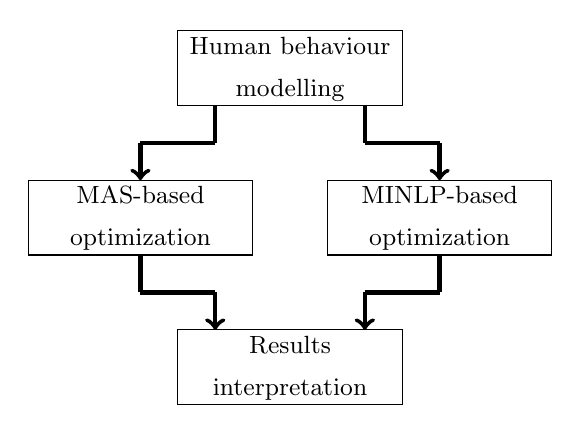
\begin{tikzpicture}[scale=0.95]
		\draw[ draw = black, fill=white](-1.5,9) rectangle (1.5,8);
		\draw (0,8.8) node{\small Human behaviour };
		\draw (0,8.2) node{\small modelling};
		\draw [draw = black, -, ultra thick] (-1,8) -- (-1,7.5);
		\draw [draw = black, -, ultra thick] (-1,7.5) -- (-2,7.5);
		\draw [draw = black, ->, ultra thick] (-2,7.5) -- (-2,7);
		\draw [draw = black, -, ultra thick] (1,8) -- (1,7.5);
		\draw [draw = black, -, ultra thick] (1,7.5) -- (2,7.5);
		\draw [draw = black, ->, ultra thick] (2,7.5) -- (2,7);
		\draw[draw = black, fill=white] (-3.5,7) rectangle (-0.5,6);
		\draw (-2,6.8) node{\small MAS-based };
		\draw (-2,6.2) node{\small optimization};
															        
		\draw [draw = black, -, ultra thick] (-2,6) -- (-2,5.5);
		\draw [draw = black, -, ultra thick] (-2,5.5) -- (-1,5.5);
		\draw [draw = black, ->, ultra thick] (-1,5.5) -- (-1,5);
															        
		\draw[draw = black, fill=white] (0.5,7) rectangle (3.5,6);
		\draw (2,6.8) node{\small MINLP-based };
		\draw (2,6.2) node{\small optimization};
		\draw [draw = black, -, ultra thick] (2,6) -- (2,5.5);
		\draw [draw = black, -, ultra thick] (2,5.5) -- (1,5.5);
		\draw [draw = black, ->, ultra thick] (1,5.5) -- (1,5);
		\draw[draw = black, fill=white] (-1.5,5) rectangle (1.5,4);
		\draw (0,4.8) node{\small Results };
		\draw (0,4.2) node{\small interpretation};
	\end{tikzpicture}\\
			
	\caption{The proposed approach}
	\label{fig:approach}
\end{figure}
	
\subsection{Simulation method}\label{sec:res1}
\subsubsection{MAS model}
To investigate and quantify the impact of human behavior on production system productivity, we developed a multi-agent systems (MAS) based simulator. The MAS comprises autonomous agents representing different elements of the real system, interacting with each other. Three interconnected agents, namely “Worker", “Job" , and “Zone", make up the simulator (see Figure~\ref{fig:interaction}.) Each agent's composition and role are defined as follows: 
\begin{itemize}
	\item Worker: it interacts with all other agents because a worker executes a job when he is on a workstation and moves between zones (productive or non-productive). The worker's parameters are:
	      \begin{itemize}
	      	\item \textit{Last\_zone}: contains the index of the last zone visited by the worker before updating his location.
	      	\item \textit{Profile}: represented by a transition probability matrix, defining movement probabilities between zones based on predefined profiles, which may differ from one worker to another.
	      	\item \textit{Next\_zone}: index of the next zone to be visited by the worker.
	      	\item \textit{Methods}: the role of the agent 'worker' is to operate the product on the machine when he is at his workstation and the product is ready. This agent moves from zone to zone according to the Markov chain model associated with his behavioral profile. The 
	      \end{itemize}
	\item Zone: This agent is a reactive agent representing workstations (WS) and non-productive zones (NPZ) located in the workshop.  
	      Each 'zone' agent is characterized by the following:
	      \begin{itemize}
	      	\item\textit{Type}: classifies the zone as \textit{productive} (a workstation) or \textit{non-productive} (e.g. infirmary, restaurant, etc.)
	      	\item\textit{Status}: status of the zone, which may be \textit{free} or \textit{occupied}. 
	      \end{itemize}
	\item Job: This agent represents the products that workers need to process, as each product passes through all workstations on the production floor. Each job is characterized by the following parameters:
	      \begin{itemize}
	      	\item\textit{Index}: the current or last workstation visited by the “Job" agent (product)
	      	\item\textit{PT}: a list of processing times at each required workstation when the worker is present
	      \end{itemize}
\end{itemize}
			      			
\begin{figure}[htbp]
	\centering
	\includegraphics[trim=00 00 00 00, clip, width=7cm]{AgentsInteractions.pdf}
	\caption{Multi-agent model's agents and their interactions}
	
	\label{fig:interaction}
\end{figure}
	
\subsubsection{System and human behavior modeling}
We consider the following production system composed of a set of $M$ workstations (WS) denoted by $\mathcal{W\!S}=\{W\!S_m, m=1,2,..,M\}$ associated with a set of workers (WK) denoted by $\mathcal{W\!K}=\{W\!K_k, k=1,2,..,K\}$.
Each workstation corresponds to a machine that needs the presence of a worker while processing a task. Each job (product) is automatically transferred to the subsequent required workstation until it completes all the necessary processing steps. Let $PT$ be the vector representing the processing times of all workstations:  
$PT=[PT_1,.., PT_m,.., PT_M]$  and let $AP$ be the vector representing the assigned workers with different behaviour profiles to workstations: $AP=[AP_1, ..., AP_k, ..., AP_K]$. 
In addition to workstations, we also define a set of $Z$ zones within the workshop where workers can go and stay for a while, making their workstation and the task that is performed on standby until they return. These zones are called “non-producible zones" (NPZ) and are denoted by $\mathcal{NPZ}=\{N\!P\!Z_z, z=1,2,..,Z\}$. The NPZ represents the areas where a worker is in a state of non-productive activity, such as a break, personal call, lunch, or simply an unjustified absence from the workstation.

We model the behavior of workers using a classical Markov chain of $Z+1$ states that correspond to the possible locations where a worker can go and stay. For each worker, the possible states (locations) belong to two classes: i) one of the $M$ ``productive" states, which corresponds to the workstation to which the worker is assigned ($p_{11}^k$), and ii) $Z$ ``non-productive" states that correspond to the NPZ (see Figure~\ref{fig:states}).

\begin{figure}[h]
	\centering\includegraphics[ clip, width=0.5\linewidth]{markovModel.pdf}

 \caption{Productive and Non-Productive States of Markovian-Based Human Behavior Model}
	\label{fig:states}
\end{figure}

We assume that each worker is assigned to a unique workstation, which does not change during the time horizon considered, and that he can only move back and forth between this workstation and the set of NPZ. The transition probabilities between each workstation and the non-productive zones are defined by the transition matrix $P^k$ relative to the $k^{th}$ generic profile of workers' behaviors.
\begin{equation}\label{eq:tmatrix}
	P^k_m =
	\left( {\begin{array}{ccccccc}
		p_{11}^k & p_{12}^k & p_{13}^k & \dots & p_{1z'}^k & \dots &p_{1(Z+1)}^k\\
		p_{21}^k & p_{22}^k & p_{23}^k & \dots & p_{2z'}^k & \dots &p_{2(Z+1)}^k\\
		p_{31}^k & p_{32}^k & p_{33}^k & \dots & p_{3z'}^k & \dots &p_{3(Z+1)}^k\\
		\vdots & \vdots & \vdots & \ddots & \vdots & \ddots & \vdots\\
		p_{z1}^k & p_{z2}^k & p_{z3}^k & \dots & p_{zz'}^k & \dots &p_{z(Z+1)}^k\\
		\vdots   & \vdots &\vdots & \ddots & \vdots & \ddots &\vdots\\
		p_{(Z+1)1}^k & p_{(Z+1)2}^k & p_{(Z+1)3}^k & \dots & p_{(Z+1)z'}^k & \dots &p_{(Z+1)(Z+1)}^k\\
		\end{array} } \right)
\end{equation}




As shown in Equation (\ref{eq:tmatrix}), ($p_{11}^k$) represents the probability that a worker with profile $k$ will remain at the workstation to which he/she is assigned, let's say $\textit{WS}_m$, $p_{1z}^k, \forall z\in \{2,..,Z+1\}$ represents the probability that a worker with profile $k$ moves from  workstation $\textit{WS}_m$ to a non-productive zone $\textit{NPZ}_z$, $p_{z1}^k$ represents the probability that a worker moves back from a nonproductive $\textit{NPZ}_z$ to his workstation $\textit{WS}_m$, and $p_{zz'}^k, \forall z,z'\in \{2,...,Z+1\} $ represents the probability of moving from $\textit{NPZ}_{z}$ to $\textit{NPZ}_{z'}$.

  


	
	
\subsubsection{Simulation procedure}
The algorithm deployed is presented in Algorithm~\ref{algo:algorithmsimulator}. When the simulation starts, three variables are initialized to zero: the simulation clock \textit{tick}, the number of completed jobs \textit{NFJ}, and the effective processing times of jobs on machines \textit{EPT}$_{jm}$. The state of the entire system is updated at each new tick until the fixed time horizon. To update the status of all agents at each time step (tick), a specific process is followed.
	    
First, all workstations are activated and their availability as well as the associated workers and operations within the input buffers $InB_{k}$ are assessed . Once these conditions are met, the value of the variable $EPT_{jm}$ increases. If $EPT_{jm}$ is equal to $PT_{m}$, it indicates that the job has been completed on the workstation $\textit{WS}_m$. The job is then moved to the input buffer $InB_{k+1}$ if the current workstation is not $\textit{WS}_K$. However, if the current workstation is $\textit{WS}_K$, the completed job $j$ is transferred to the output buffer $OutB$ of that workstation (last workstation). If the current workstation is $\textit{WS}_1$, a new job is generated. 

During this process, the worker is not present all the time on his workstation, but follows the Markovian process to move between the productive zone (his workstation) and non productive zones (break, nursery, lunch). In this model, the behavior of worker is completely independent from its environment, where the production operations can be interrupted when the transition to a new position is generated by the Markov chain model.   

\begin{algorithm2e}[H]  
\algsetup{linenosize=\tiny}
  \scriptsize
	\KwData{}	 
	\ \ $\mathcal{WK}=\{WK_1, WK_2,.., WK_K\}$: Set of workers\;
	\ \ $\mathcal{WS}=\{WS_1,WS_2,..,WS_M\}$: Set of workstations\;
	\ \ $\mathcal{J}=\{1,..,J\}$: Set of jobs indices\;
	\ \ $\mathcal{K}=\{1,..,K\}$: Set of workers' (workstations) indices\;
	\ \ $PT=(PT_{m}:  m\in\mathcal{M})$: Processing times vector\;
	\ \ $InB=(InB_m: m\in\mathcal{M})$: Workstations' input buffers\;
	\ \ $OutB$: Output buffer of completed jobs (buffer of the last workstation)\;
	\ \ $Horizon$: Simulation horizon\;
	\ \  $EPT_{jm}$: the effective processing time of the job $j$ on the Workstation $m$ \;
	\ \ $tick$: unit of time that passes between iterations of the simulation \;
	\KwResult{}
	\ \ \it{NFJ}: Number of finished jobs  \; 
	\ \ $Productivity$: Productivity rate  \;
	\Begin{
		Initialization: $tick=1$ , \quad  \it{NFJ}$=0$ , \quad  \it{EPT}$_{jm}=0 \quad  \forall j\in\mathcal{J} \  \forall m\in\{1,..,M\}$\;
		\While{$tick <= Horizon$}{
			
			Update workers' locations\;
			\For{Each  $WS_m\in\mathcal{WS}$}{
   \For{Each  $WK_k\in\mathcal{WK}$}{
				\If{($WS_m$ is occupied by $j\in\mathcal{J}$ \textbf{AND} $WK_k$ is present) \textbf{OR} ($WS_m$ NOT occupied \textbf{AND} \ $\exists j\in\mathcal{J}$ in $InB_m$ \textbf{AND} $WK_m$ is present)}{
					$EPT_{jm}  \leftarrow	  EPT_{jm}+1$ \; 
					\If{$EPT_{jm} = PT_{jm}$ }{
						\eIf{$m =M$ }{
							Transfer job $j$ to $OutB$ \;
							$NFJ \leftarrow NFJ+1$\;
						}
						{
							Transfer job $j$ to $InB_{m+1}$\;
							\If{m=1}{
								Generate a new job at $WS_1$
							}
						} 
					}
				}
			}}
        $tick\leftarrow tick+1$\;		
  }
		$Productivity\leftarrow \frac{NFJ}{Horizon}$\;
	}
	\caption{Simulation algorithm}
            \label{algo:algorithmsimulator}
\end{algorithm2e}	   

        
				
\subsection{Optimization model}\label{sec:Pre_mod}
In this section, we introduce our non-linear optimization model designed to identify the most efficient worker-to-machine assignment, ultimately maximising productivity for the dual resource flow shop production system. 
	
\subsubsection{Notations}
\begin{longtable}{p{.08\textwidth} p{.92\textwidth}}
	\hline
	\multicolumn{2}{c}{Sets }\\
	\hline
	$\mathcal{M}$ & set of workstations (productive zones), with $|\mathcal{M}|=M$                      \\
	$\mathcal{T}$ & set of  product types	with $|\mathcal{T}|=T$                                                                                                                                                                                           \\
	$\mathcal{K}$ & set of workers, with $|\mathcal{K}|=K$                                                                                                                                                                                                 \\
	$\mathcal{P}$ & set of worker profiles available on the job market, with $|\mathcal{F}|=P$                                                                                                                                                             \\	      		\hline
	\multicolumn{2}{c}{Indices }\\
	\hline
	$m$           & indices of workstations, with $m\in\{1,2,..,M\}$                                                                                                                                                                                       \\
	$j$           & indices of jobs, with $j\in\{1,2,..,J\}$                                                                                                                                                                                               \\
	$t$           & indices of job types (product) , with $t\in\{1,2,..,T\}$                                                                                                                                                                               \\
	$k$           & indices of workers, with $k\in\{1,2,..,K\}$                                                                                                                                                                                            \\
	$p$           & indices of profiles, with $p\in\{0,1,2,..,P-1\}$                                                                                                                                                                                       \\
	\hline
	\multicolumn{2}{c}{Parameters}\\
	\hline
	$H$           & time horizon of production                                 \\
	$I$           & production mix, with $I=(I_1,I_2,..,I_t,..,I_T)$ where $I_t$ is the minimum demand for the type of product $t$ and .                                                                                                                   \\
	$f_{k,p}$     & a binary variable indicating whether the worker $k$  belongs to the profile $p$, where each worker can get only one profile $\sum_{p\in\mathcal{P}} f_{p,k} =1  \quad\forall k\in\mathcal{K}$                                          \\
	$\lambda^1_p$ & average duration of the working time period of the workers of the profile $p$                                                                                                                                                          \\
	$\lambda^0_p$ & average duration of the absence time period of the workers of the profile $p$                                                                                                                                                          \\
	$\tau_{t,m}$  & reference processing time of the product type $t$ on workstation $m$                                                                                                                                                                   \\
	$\alpha_k$    & average continuous working time of the worker $k$                                                                                                                                                                                      \\
	$\gamma_k$    & average absence time of the worker $k$ after a period of working time                                                                                                                                                                  \\
	$J$           & the maximum number of products (all types combined) that can be produced:                                                                                                                                                              \\
											
	              & $J=\displaystyle\max_{t\in{\cal T}}\left\lceil {(H-\sum_{m\in\mathcal{M}} \tau_{t,m})}/{\max_{m\in\mathcal{M}} \tau_{t,m}}\right\rceil$, where $\left\lceil x    \right\rceil $   is the smallest integer greater than or equal to $x$ \\
	$HV$          & a high value number                                                                                                                                                                                                                    \\
	\hline
	\multicolumn{2}{c}{Decision variables }\\
	\hline		
	$X_{t,j}$     & a binary variable indicating if the $j$-th job is a product of type $t$                                                                                                                                                                                  \\
	$Y_j$         & a binary variable indicating the launch of the $j$-th job, i.e. equals 1 if the product is assigned to a product type, 0 otherwise:                   $Y_j = {\sum_{t\in \mathcal{T}} X_{t,j}} \quad\forall{j \in\mathcal{J} }$                                                                                                                                                              \\
	$W_{k,m}$     & a binary variable indicating if the worker $k$ is assigned to the workstation $m$                                                                                                                                                      \\
	$N_{j,m}$     & the number of interruptions (due to the absence of worker) to the job $j$ on workstation  $m$                                                                                                                                      \\
	$U_m$         & the average continuous productivity time (up-time) of the workstation $m$:                                                                                                                                                             \\ 
	              & $U_m=\sum_{k\in \mathcal{K}} \alpha_k \times W_{k,m} \quad \forall{ m \in  \mathcal{M}}$                                                                                                                                               \\
	$D_m$         & the average continues non-productivity time (downtime) of the workstation $m$:                                                                                                                                                         \\
	              & $D_m = \sum_{k\in\mathcal{K}} \gamma_k \times W_{k,m} \quad\forall m\in\mathcal{M}$                                                                                                                                                    \\
	$\Pi_{j,m}$   & the effective processing time of the job $j$ at the machine $m$. It includes the real processing time and the absence time of the operator:                                                                                            \\
	              & $\Pi_{1,m} = N_{1,m}\times D_m  + \sum_{t\in\mathcal{T}} ( X_{t,1} \times\tau_{t,m}) \quad \forall m\in\mathcal{M} $                                                                                                                   \\
	              & $\Pi_{j,m} =  (N_{j,m}-N_{j-1,m})\times D_m + \sum_{t\in \mathcal{T}}( X_{t,j} \times \tau_{t,m}  )\quad\forall{j=2..J} \quad  \forall m\in\mathcal{M}$                                                                                \\
	$C_{j,m}$     & the completion time of the job $j$ on workstation  $m$                                                                                                                                                                                 \\
	$\Pi^C_{j,m}$ & the cumulative processing time to the job $j$ at the machine $m$                                                                                                                                                                       \\
	              & $\Pi^C_{1,m} = \sum_{t\in \mathcal{T}} (X_{t,1} \times\tau_{t,m})\quad\forall m \in\mathcal{M}$                                                                                                                                        \\
	              & $\Pi^C_{j,m} =\Pi^C_{j-1,m} +  \sum_{t\in \mathcal{T}} (X_{t,j} \times \tau_{t,m} )   \quad\forall j=2..J \quad\forall m \in\mathcal{M}$                                                                                               \\
										
	\hline
\end{longtable}		
	
\begin{figure}[htbp]
	\centering
	\rotatebox{0}{\includegraphics[width=12cm]{ModelVariablesLinks.pdf}}
	\caption{Mathematical model's data and variables and their links}
			    
			
	\label{fig:ModelVariablesLinks2}
\end{figure}
					
					              
\subsubsection{Problem formulation}
					
			
					
The dual-resource constrained flow-shop worker assignment and scheduling problem is formalised by Mixed Integer Nonlinear Programming  model:
\begin{equation}
	\text{{\it obj}: Maximize } \sum_{j=1..J}Y_j\label{obj1}
\end{equation} 
			
The objective of our model is to maximize the productivity of the production system across a finite time horizon for all types of products. Therefore, the objective function in Eq.~(\ref{obj1}) aims to Maximize the total number of finished products during the considered time horizon. Alternatively, the objective function could be to minimise the makespan of a given number of demanded products. However, we choose to Maximize the throughput to facilitate comparison with the simulation part and obtain a stable comparison between different scenarios.
	
This objective function is subject to the following constraints:
\begin{spacing}{.5}	
	\begin{equation}
		\begin{array}{ll}		
			  &   
		\end{array}
		{{\sum_{k\in \mathcal{K}}W_{k,m}}=1 \quad \forall{ m \in  \mathcal{M}}}
		\label{c3}
	\end{equation}
	\begin{equation}
		\begin{array}{ll}
			  &   
		\end{array}
		{{\sum_{m\in \mathcal{M}}W_{k,m}}\leq 1 \quad \forall{ k \in  \mathcal{K}}}
		\label{c4}
	\end{equation}
	\begin{equation}\label{c5}
		X_{t,j}  \leq 1  \quad\forall j \in \{1,...,J\}\quad\forall{t\in\mathcal{T}}
	\end{equation} 
	\begin{equation}\label{c6}
		X_{t,j}  \leq I_t  \quad\forall j \in \{1,...,J\} \quad \quad\forall{t\in\mathcal{T}}
	\end{equation} 
	\begin{equation}\label{c7}
		{{\sum_{j=1..J} X_{t,j} }   \geq I_t   \quad \quad\forall{t\in\mathcal{T}}}
	\end{equation} 
	\begin{equation}\label{c8}
		\text{\quad }  Y_j\leq Y_{j-1} \quad\forall j \in \{2,...,J\}
	\end{equation}									 
	\begin{equation}\label{c9} 
		N_{j,m} +1 \geq \frac{\Pi_{j,m}}{U_m}  \quad\forall j \in \{1,...,J\}  \quad\forall m\in\mathcal{M}
	\end{equation}
											
	\begin{equation}\label{c10} 
		N_{j,m}  + 0.001  \leq \frac{\Pi_{j,m}}{U_m}  \quad\forall j \in \{1,...,J\} \quad\forall m\in\mathcal{M}
	\end{equation}
											 
	\begin{equation}\label{c11}
		C_{1,1} = \Pi_{1,1} 
	\end{equation}
																				
	\begin{equation}\label{c12}
		C_{j,m} \geq Y_j\times\Pi_{j,m}+C_{j-1,m}\quad\forall j \in \{2,...,J\}\quad\forall{m\in\mathcal{M}}
	\end{equation} 
	\begin{equation}\label{c13}
		C_{j,m} \geq Y_j\times\Pi_{j,m}+C_{j,m-1}  \quad\forall j \in \{1,...,J\} \quad\forall m \in \{2, ..., M\}
	\end{equation} 			
	\begin{equation}\label{c14}
		C_{j,m} \leq H\quad\forall j \in \{1,...,J\}\quad\forall{ m \in\mathcal{M}} 
	\end{equation} 	
						
\end{spacing}
					
	
Constraints (\ref{c3}) and (\ref{c4}) ensure that each machine is assigned to one worker and that each worker is assigned to at most one machine. 
Constraints (\ref{c5}) and (\ref{c6}) ensure that the production mix is respected by producing only types of products $t\in\mathcal{T}$ such as $I_t >= 1$.
Constraints (\ref{c7}) ensure that the minimum production mix is respected.
Constraints (\ref{c8}) ensure a strict production sequence, where the product $j$ is not produced unless the previous product $j-1$ has already been produced, by allowing the indexing of manufactured products in ascending order.
Non-linear constraints (\ref{c9}) and (\ref{c10}) link the actual duration of each job on a given machine with the number of interruptions, the average uptime, and the average downtime, which depend on the profile of the worker assigned to the machine.  
Finally, constraints (\ref{c11}), (\ref{c12}), (\ref{c13}) and (\ref{c14}) guarantee that precedence constraints are respected between operations of the same product and that the last operation of the last planned product is completed before the end of the planning horizon $H$.
	
Figure~\ref{fig:ModelVariablesLinks2} illustrates the different constraints and the relationship between the parameters and decision variables of the model. To demonstrate the functioning of the model, we developed an illustrative model, which will be explained in the following section.
					
			
					
\subsubsection{Illustrative example}
In this example, we have a three-step flow-shop production system with five workers, where $M=3$ and $K=5$. The system is capable of manufacturing three types of products ($T=3$) with varying processing times on each workstation (machine). The workers' behaviours are categorized into three generic behavioural profiles (${\cal P}={p_1,p_2,p_3}$), which are characterized by their average absence times $(\lambda^0_{p_1},\lambda^0_{p_2},\lambda^0_{p_3})$ and average working times $(\lambda^1_{p_1},\lambda^1_{p_2},\lambda^1_{p_3})$. For each profile $p$, $\lambda^0_{p}$ and $\lambda^1_{p}$ represent the expected sojourn times in “non-productive" states/zones (NPZs) and the “productive" state (workstation), respectively, calculated from the Markov transition probability matrix of the corresponding profile. The parameters $\gamma_k$ and $\alpha_k$ for each worker $k$ are randomly generated using exponential distributions with parameters $\sum_{p\in\mathcal{P}}f_{k,p}\lambda^0_p$ and $\sum_{p\in\mathcal{P}}f_{k,p}\lambda^1_p$, respectively.  
					
The optimal solution is illustrated in Figure~\ref{fig:Ex_p3}, which presents the optimal values of all decision variables and the objective function. The matrix $X^*$ indicates that, at most, five products can be scheduled within the imposed time horizon, consisting of 2 products of type $t1$, 1 product of type $t_2$, and 4 products of type $t_3$. The optimal assignment of workers is provided in matrix $W^*$, where workers $k_2$, $k_3$, and $k_5$ are assigned to workstations $\textit{WS}_3$, $\textit{WS}_2$, and $\textit{WS}_1$, respectively. The Gantt chart displaying the optimal schedule is shown in Figure~\ref{fig:Ex_p4}.
			
\begin{figure}[htbp]
	\centering
	\rotatebox{0}{\includegraphics[width=\textwidth]{Example.pdf}}
	\caption{different values relation of decision variables and parameters of the illustrative example }
	
	\label{fig:Ex_p3}
\end{figure}
					
Consider the optimal solution generated by the optimization process. By combining the assignments of the workers $W^*_{k,m}$ with their respective profiles $f_{k,p}$, we are able to obtain the ideal assignment of profiles to workstations, represented by \quad $M^*_{p,m}=\quad \sum_{k \in \mathcal{K}} W^*_{k,m} f_{k,p} \quad \forall{p\in \mathcal{P},m \in \mathcal{M}} $. This optimal assignment not only Maximizes efficiency of the production system, but also ensures that each worker is assigned to a task that best aligns with their particular behaviour. To show the efficiency of the model in the case of several products, we set the minimum demand $I$ . 
To better understand and verify the results, we present the Gantt chart of the optimal solution obtained in Figure~\ref{fig:Ex_p4}. The production horizon is limited to 26 time periods, within which seven jobs are processed. The optimization algorithm has assigned worker k=5, belonging to profile~2, to workstation~1, worker~3, belonging to profile~3, to workstation~2, and worker~2, belonging to profile~1, to workstation~3. Furthermore, the algorithm schedules the jobs by starting with three jobs of type~3 (in blue), followed by one job of type~1 (orange), one job of type~2 (green), one job of type~1 (orange), and finally, the last job of type~2 (green).
	
Different times used for the implementation of the algorithm are illustrated, such as processing time ($\tau_{t,m}$), completion time ($C_{j,m}$), and cumulative processing time ($\Pi^C_{j,m}$). This example demonstrates that the proposed model provides a feasible and logic solution that takes into account different human profiles and different workers belonging to different profiles.  
					
\begin{figure}[htbp]
	\centering
	\rotatebox{0}{\includegraphics[width=\textwidth]{EX_Gantt.pdf}}
	\caption{Gantt chart of the obtained solution of the illustrative example}
	\label{fig:Ex_p4}
\end{figure}
									
\section{Numerical experiments and discussion}\label{sec:Exp_dis}
\subsection{Simulation results}
We employed the NetLogo 6.2.1 software, equipped with its own programming language designed for multi-agent modelling systems, to develop the simulator based on our MAS model (see Figure~\ref{fig:simulator}). Our simulations were based on an example inspired by a case study of the annual preparation of educational robots used in the robotics practical works of a French engineering school. The simulation represented a flow-shop production system consisting of six workstations in the productive zone and three non-productive zones that represent reasons for workers to temporarily leave their workstation, such as a personnel call, lunch break, or treatment in the infirmary as presented in Figure~\ref{fig:simulator}. Each worker was responsible for performing one or several specific production operations using a set of equipment associated with their workstation. The use of the simulator allows us to show the movement of workers that can move between the workstations ($WS_i$) and the nonproductive zones. The product represented by boxes moving through the production line. Their transformation is represented by a modification of the colour of the product from black to white.
\begin{figure}[htbp]
	\centering
	\includegraphics[width=10cm]{simulation.png}
	\caption{Overview of the simulation environment}
	\label{fig:simulator}
\end{figure}
		
To study the impact of different human behaviours on the productivity of dual-resource (human and machine) production systems, we conducted multiple simulations using a Markov chain-based model of human behaviour within a multi-agent system (MAS). In each simulation, the workers were assigned specific operations based on their workstation, and their movements between 'productive' and 'nonproductive' states were determined by their behavioural profile.
	
Six different profiles of worker behaviour were proposed based on empirical observations, each represented by a Markov chain with its own transition matrix. These matrices were used to differentiate between the various worker profiles. The six generic profiles of worker behaviour were represented by the following Markov chain transition matrices:
\counterwithout{table}{section}
\begin{table}[htbp] 
	\centering
	\begin{tabular}{ccc}
		& & \\
		$ P^0 = \left( {\begin{array}{cccc}
		1    & 0    & 0   & 0   \\
		1    & 0    & 0   & 0   \\
		1    & 0    & 0   & 0   \\
		1    & 0    & 0   & 0   \\
		\end{array} } \right)$ 
		&
		$P^1 = \left({\begin{array}{cccc}
		0.95 & 0.05 & 0   & 0   \\
		0.95 & 0.05 & 0   & 0   \\
		1    & 0    & 0   & 0   \\
		1    & 0    & 0   & 0   \\
		\end{array} } \right)$  \\
		& \\
		$P^2 = \left( {\begin{array}{cccc}
		0.9  & 0.1  & 0   & 0   \\
		0.95 & 0.05 & 0   & 0   \\
		1    & 0    & 0   & 0   \\
		1    & 0    & 0   & 0   \\
		\end{array} } \right)$ 
		&
		$P^3 = \left( {\begin{array}{cccc}
		0.7  & 0.3  & 0   & 0   \\
		0.95 & 0.05 & 0   & 0   \\
		1    & 0    & 0   & 0   \\
		1    & 0    & 0   & 0   \\
		\end{array} } \right)$ \\
		& \\
		$P^4 = \left( {\begin{array}{cccc}
		0.7  & 0.3  & 0   & 0   \\
		0.7  & 0.3  & 0   & 0   \\
		1    & 0    & 0   & 0   \\
		1    & 0    & 0   & 0   \\
		\end{array} } \right)$ 
		&
		$P^5 = \left( {\begin{array}{cccc}
		0.8  & 0.2  & 0   & 0   \\
		0.6  & 0.2  & 0.1 & 0.1 \\
		0    & 0.3  & 0.4 & 0.3 \\
		0    & 0.3  & 0.3 & 0.4 
		\end{array} } \right)$    
					
	\end{tabular}\\
	\label{tab:mytable}
\end{table}			
Each Markov chain consists of four states, which are determined by the workers' positions and activities. The workers can either be in a productive zone, where they are working at their assigned workstations (PZ), or a non-productive zone (NPZ). The NPZ is where workers can be found taking a coffee or lunch break, making a personal call or taking a bathroom break, or being in the infirmary for care.
	
The transition probabilities between these states differ depending on the worker profile. The profiles considered in the simulation aim to cover all possible situations, ranging from the “as-robot" profile ($P^0$), where the worker does not move from the working zone, to the 'undisciplined/disruptive' profile such as profile $P^5$. Other input parameters used in the simulation are as follows:
\begin{itemize}
	\item Simulation time horizon: 1 week of 5 working days, 8 hours per day
	\item Workstations' processing times:\\ $PT=[1,4,2,4,1,3]$ for the workstations $\textit{WS}_1$ to $\textit{WS}_6$, respectively.
	\item Workers' profiles: $P^0$ (Ideal), $P^1$, $P^2$, $P^3$, $P^4$ and $P^5$ 
	\item Scenarios of profiles assignment: we simulated 36 scenarios, representing  different combinations of workers' profiles assigned to workstations.\\
 \begin{itemize}
    \item  \textit{Global scenarios (6)}:
    \begin{itemize}
        \item 	      \hspace*{0.5cm} G0: $AP=[0,0,0,0,0,0]$ (Perfect)
	\item    \hspace*{0.5cm} Gk: $AP=[k,k,k,k,k,k]$, $k=1,2,..,5$ 
    \end{itemize}

    \item  \textit{Mixed scenarios (30)}: 
    \begin{itemize}
        \item 	  \hspace*{0.5cm} Mk1: $AP=[k,0,0,0,0,0]$, $k=1,2,..,5$
	\item     \hspace*{0.5cm} Mk2: $AP=[0,k,0,0,0,0]$, $k=1,2,..,5$
	  \item    \hspace*{0.5cm} Mk3: $AP=[0,0,k,0,0,0]$, $k=1,2,..,5$
	  \item    \hspace*{0.5cm} Mk4: $AP=[0,0,0,k,0,0]$, $k=1,2,..,5$
	  \item    \hspace*{0.5cm} Mk5: $AP=[0,0,0,0,k,0]$, $k=1,2,..,5$
	  \item    \hspace*{0.5cm} Mk6: $AP=[0,0,0,0,0,k]$, $k=1,2,..,5$
    \end{itemize}

 \end{itemize}
	     
	\item Gk: value of the Global scenarios
	\item {\it{\%gap}}  :  The percentage gap of the productivity of a given scenario ($\pi(s)$) compared to a reference scenario ($\pi(s^0)$),  $\textit{\%gap}=\frac{\pi(s^0) - \pi(s)}{\pi(s^0)}$.
\end{itemize}
\setcounter{table}{0}
\begin{table}[htbp] 
	\begin{center}
					
					   
		\begin{longtable}{cc|cccccc|ccc|}
			\hline
			\multicolumn{2}{c|}{Scenarios} & \multicolumn{6}{c|}{Operator profiles assignment}& \multicolumn{2}{c}{Productivity (u)}&\\
   % (u/wk)
			\# & ID  & $\textit{WS}_1$ & $\textit{WS}_2$ & $\textit{WS}_3$ & $\textit{WS}_4$ & $\textit{WS}_5$ & $\textit{WS}_6$ & 
			& Gk   & \it{\%gap} \\ 
			\hline
			1  & G0  & 0 & 0 & 0 & 0 & 0 & 0 & 597 & -   & -    \\
			2  & G1  & 1 & 1 & 1 & 1 & 1 & 1 & 564 & -   & -    \\
			3  & G2  & 2 & 2 & 2 & 2 & 2 & 2 & 564 & -   & -    \\
			4  & G3  & 3 & 3 & 3 & 3 & 3 & 3 & 533 & -   & -    \\
			5  & G4  & 4 & 4 & 4 & 4 & 4 & 4 & 533 & -   & -    \\
			6  & G5  & 5 & 5 & 5 & 5 & 5 & 5 & 563 & -   & -    \\
			\hline
			7  & M11 & 1 & 0 & 0 & 0 & 0 & 0 & 597 & 564 & 5.9  \\
			8  & M12 & 0 & 1 & 0 & 0 & 0 & 0 & 567 & 564 & 0.5  \\
			9  & M13 & 0 & 0 & 1 & 0 & 0 & 0 & 597 & 564 & 5.9  \\
			10 & M14 & 0 & 0 & 0 & 1 & 0 & 0 & 567 & 564 & 0.5  \\
			11 & M15 & 0 & 0 & 0 & 0 & 1 & 0 & 597 & 564 & 5.9  \\
			12 & M16 & 0 & 0 & 0 & 0 & 0 & 1 & 597 & 564 & 5.9  \\
			\hline
			13 & M21 & 2 & 0 & 0 & 0 & 0 & 0 & 597 & 564 & 5.9  \\
			14 & M22 & 0 & 2 & 0 & 0 & 0 & 0 & 567 & 564 & 0.5  \\
			15 & M23 & 0 & 0 & 2 & 0 & 0 & 0 & 597 & 564 & 5.9  \\
			16 & M24 & 0 & 0 & 0 & 2 & 0 & 0 & 567 & 564 & 0.5  \\
			17 & M25 & 0 & 0 & 0 & 0 & 2 & 0 & 597 & 564 & 5.9  \\
			18 & M26 & 0 & 0 & 0 & 0 & 0 & 2 & 597 & 564 & 5.9  \\
			\hline
			19 & M31 & 3 & 0 & 0 & 0 & 0 & 0 & 597 & 533 & 12.0 \\
			20 & M32 & 0 & 3 & 0 & 0 & 0 & 0 & 535 & 533 & 0.4  \\
			21 & M33 & 0 & 0 & 3 & 0 & 0 & 0 & 597 & 533 & 12.0 \\
			22 & M34 & 0 & 0 & 0 & 3 & 0 & 0 & 537 & 533 & 0.8  \\
			23 & M35 & 0 & 0 & 0 & 0 & 3 & 0 & 597 & 533 & 12.0 \\
			24 & M36 & 0 & 0 & 0 & 0 & 0 & 3 & 597 & 533 & 12.0 \\
			\hline
			25 & M41 & 4 & 0 & 0 & 0 & 0 & 0 & 597 & 533 & 12.0 \\
			26 & M42 & 0 & 4 & 0 & 0 & 0 & 0 & 537 & 533 & 0.8  \\
			27 & M43 & 0 & 0 & 4 & 0 & 0 & 0 & 597 & 533 & 12.0 \\
			28 & M44 & 0 & 0 & 0 & 4 & 0 & 0 & 538 & 533 & 0.9  \\
			29 & M45 & 0 & 0 & 0 & 0 & 4 & 0 & 597 & 533 & 12.0 \\
			30 & M46 & 0 & 0 & 0 & 0 & 0 & 4 & 597 & 533 & 12.0 \\
			\hline
			31 & M51 & 5 & 0 & 0 & 0 & 0 & 0 & 597 & 563 & 6.0  \\
			32 & M52 & 0 & 5 & 0 & 0 & 0 & 0 & 566 & 563 & 0.5  \\
			33 & M53 & 0 & 0 & 5 & 0 & 0 & 0 & 597 & 563 & 6.0  \\
			34 & M54 & 0 & 0 & 0 & 5 & 0 & 0 & 568 & 563 & 0.9  \\
			35 & M55 & 0 & 0 & 0 & 0 & 5 & 0 & 597 & 563 & 6.0  \\
			36 & M56 & 0 & 0 & 0 & 0 & 0 & 5 & 597 & 563 & 6.0  \\
			\hline
            \\
		\end{longtable}
            
		\caption{Results of all tested scenarios (Simulation)}
		\label{tab:t0}
	\end{center}

\end{table}
	
Table~\ref{tab:t0} presents the simulation results, showing the level of productivity achieved by each scenario. Out of 35 scenarios, 20 performed equally well as the perfect scenario where all workers have the ideal profile.
\\
This finding suggests that the impact of each profile on productivity can vary depending on the workstation to which it is assigned. Further examination of the results reveals that the productivity level decreases significantly when profiles \#3 or \#4 are assigned to bottleneck workstations such as $\textit{WS}_2$ or $\textit{WS}_4$. Therefore, it is evident that the allocation of workers to specific workstations affects productivity, and careful consideration of the profiles of the workers is necessary to optimize overall productivity.
	
Based on the results, we will attempt to discuss the effect of operator placement on the production line and how one can benefit from the performance difference to place these operators in a favorable position.


\begin{figure}[htbp]
	\centering	    
										
	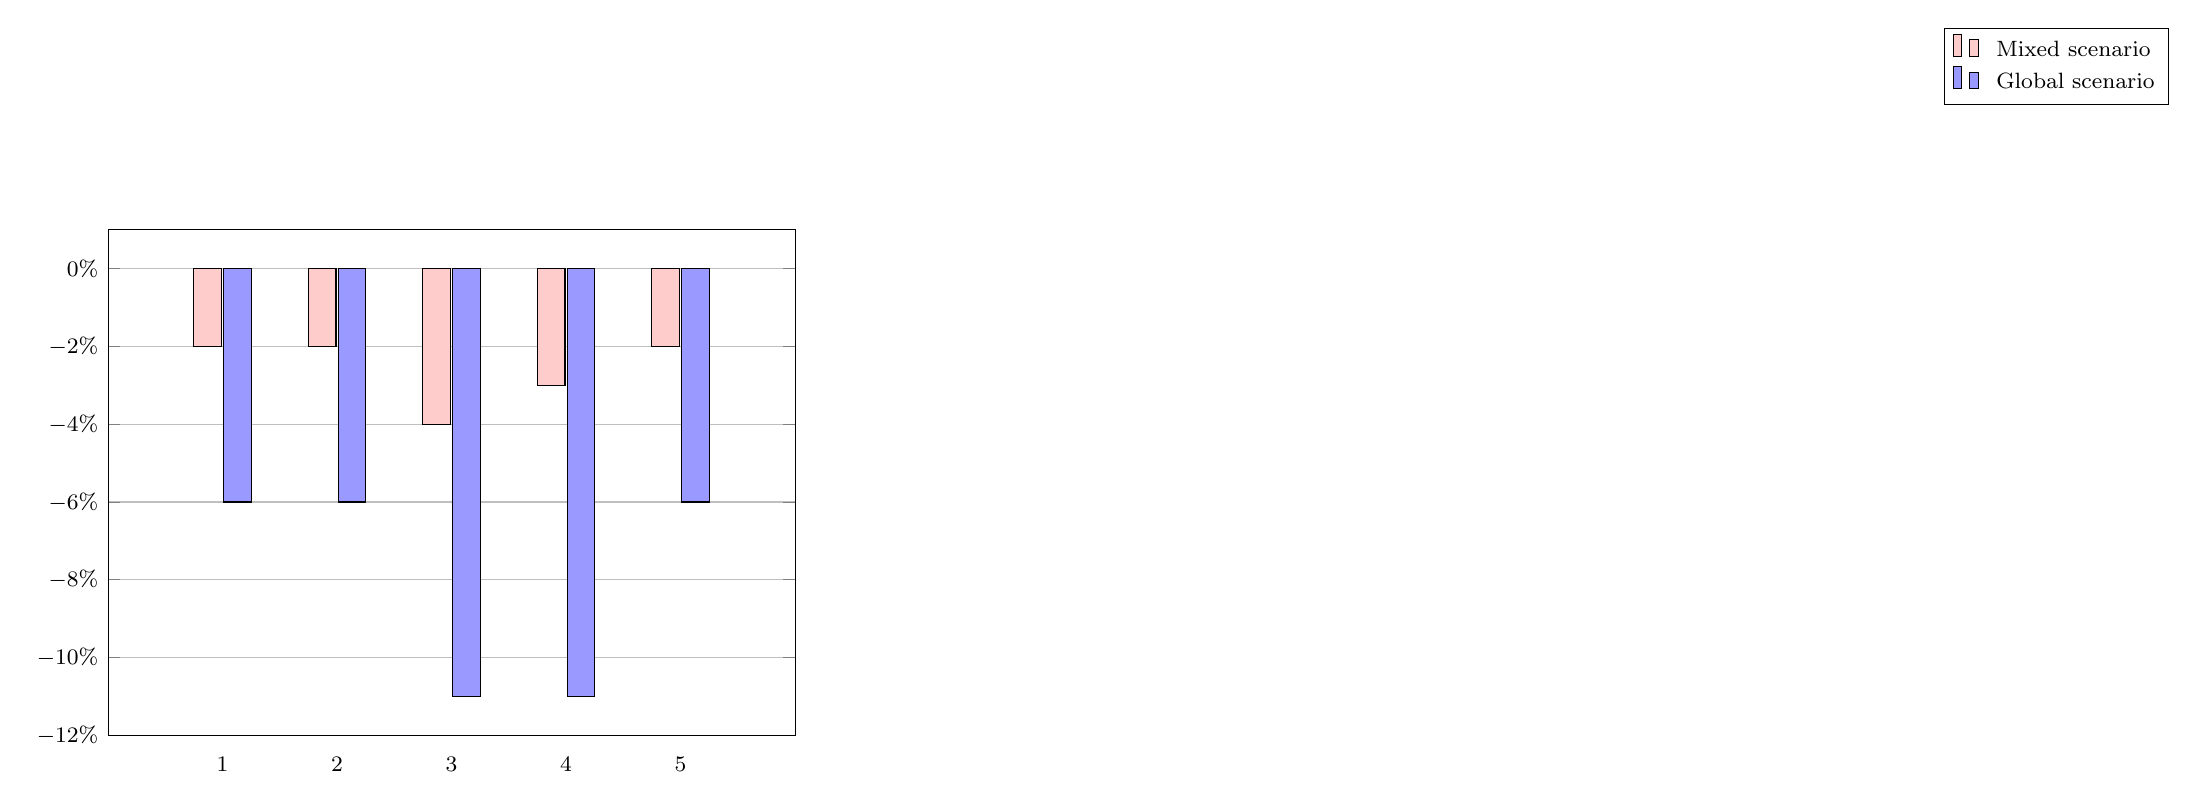
\begin{tikzpicture}[font=\footnotesize,baseline]
		\begin{axis}[
				width  = 0.85*\textwidth,
				height = 8cm,
				major x tick style = transparent,
				ybar=2*\pgflinewidth,
				bar width=10pt,
				ymajorgrids = true,
				ymin=-12,
				ymax=1,
				yticklabel={\pgfmathparse{\tick}\pgfmathprintnumber{\pgfmathresult}\%},
				xtick = data,
				scaled y ticks = false,
				enlarge x limits=0.25,
				legend cell align=left,
				legend entries={Mixed scenario, Global scenario},
				legend style={
					at={(3,1.4)},
					anchor=north east,
					column sep=1ex
				}
			]								
			\addplot[color=black, fill=red!20,mark=none] coordinates {(1,-2)(2,-2)(3,-4)(4,-3)(5,-2)};
			\addplot[color=black,fill=blue!40,mark=none] coordinates {(1,-6)(2,-6)(3,-11)(4,-11)(5,-6)};
		\end{axis}
		\ref{named}
	\end{tikzpicture}
	\caption{Effect of profile assignment strategies on productivity}
	\label{fig:glo_mix}
\end{figure}

Figure~\ref{fig:glo_mix} displays the percentage decrease in productivity, compared to the perfect profile, 
for each profile in both mixed scenarios (on average) and global scenarios. For example, if profile \#2 is assigned to all workstations (global scenario), there is a reduction 6\% in productivity compared to the perfect profile (green bar). However, in the mixed scenario, this reduction drops to an average of 2\% (red bar).
	
The profile with the highest average slowdown in productivity is \#4 and  \#3, which results in a 11\% reduction. This is because the probability of staying at a workstation is only $0.7$ in the corresponding Markov chain.

Based on the results above, we can define for each profile a ranking of workstations assignment regarding the throughput performance. The ideal worker profile is ranked first for all workstations, which means that we obtain the maximum throughput when it is placed in any workstation. The other worker profile are reducing the throughput when they are placed on the bottleneck stations (\#2 and \#4). For profile $P_1$ and $P_2$, the assignment of the worker to $\textit{WS}_1$, $\textit{WS}_3$,$\textit{WS}_5$, or $\textit{WS}_6$ is giving the maximum throughput of 597 (Rank1), followed by  $\textit{WS}_2$, and  $\textit{WS}_4$ with a throughput of 567 (Rank2).  Similarly, Profiles $P_3$, $P_4$, and $P_5$ are best ranked with workstations $\textit{WS}_1$, $\textit{WS}_3$,$\textit{WS}_5$, or $\textit{WS}_6$ that have the lowest processing time, and obtaining a rank 2 when assigned to $\textit{WS}_4$ with a throughput of 538, it also obtains the rank 3 when assigned to the $\textit{WS}_2$ with a throughput of 537.
	
Although the chosen scenarios are very restrictive, these results demonstrate how human behaviour can negatively impact productivity and highlight the importance of an optimized allocation of different worker profiles to workstations. To address this issue, the following section proposes an effective optimization method for selecting the most suitable allocation of a group of workers with diverse behavioural profiles to a given number of workstations.


\subsection{Optimisation results}
The mathematical model presented in the previous section has been implemented using the Python and Gurobi optimization solver library. 
We conducted experiments using the same instance as the experiments using the simulation method described in the previous section, which included six workstations and six distinct behavioural profiles of workers. Furthermore, we considered four different types of product in our analysis $\{t_1, t_2, t_3\}$. The processing times $\tau_{t,m}$ of each product type on each workstation are given as follows:

	 
\begin{itemize}
	\item $t_1$ : $\textit{WS}_1(1)$ , $\textit{WS}_2(4)$ , $\textit{WS}_3(2)$ , $\textit{WS}_4(4)$ , $\textit{WS}_5(1)$ ,$\textit{WS}_6(3)$ with a nominal cycle time of 4
	\item $t_2$ : $\textit{WS}_1(2)$ , $\textit{WS}_2(1)$ , $\textit{WS}_3(2)$ , $\textit{WS}_4(1)$ , $\textit{WS}_5(4)$ ,$\textit{WS}_6(3)$ with a nominal cycle time of 4
	\item $t_2$ : $\textit{WS}_1(1)$ , $\textit{WS}_2(3)$ , $\textit{WS}_3(3)$ , $\textit{WS}_4(3)$ , $\textit{WS}_5(3)$ ,$\textit{WS}_6(3)$ with a nominal cycle time of 3
\end{itemize}
					
To capture the potential variability in worker profiles and production mix, we defined 75 unique scenarios, each with varying numbers of workers belonging to each profile and production mix. These scenarios were then organised into nine distinct groups, labelled “GA" to “GI", as follows:
\begin{itemize}
	\item In the Group A scenarios, six workers with the same profile are assigned to test the overall impact of this profile on
	      +productivity and to classify the profiles. 
	\item In the scenarios of Group B, 5 workers with profile 0 (perfect profile) and 1 worker with a different profile are assigned to deduce the partial impact of each profile on each machine.
	\item In the scenarios of Groups C, D, E, and F, the same strategy as in Scenario B is adopted, but with a gradual decrease in the number of workers with profile 0. This will allow testing the partial effect of each profile, while the other machines are perfect. 
	\item The scenario of Group G is a scenario in which the profiles were randomly selected to study the impact of a combination of profiles on productivity.
	\item  In all scenarios (A to G), only the production of a type 1 product is allowed in order to test only the effect of the worker allocation on the productivity of the system.
	\item In scenarios of Group H, we allow the production of several types of product to test the effect of profile allocation and scheduling of jobs on the productivity of the system.  
\end{itemize}
					
In order to assess the efficiency of the optimal solution, the latter is compared to the “the worst assignment" solution for each scenario. The worst assignment of workers to jobs is achieved by iteratively assigning the most undisciplined worker (highest ratio $\lambda^0_p/(\lambda^0_p+\lambda^1_p)$) to the most important production machine (bottleneck) and vice versa.
					
Each scenario runs on a time horizon of one week of five working days, eight hours per day, that is, $H=2400$ hours. The result of each tested scenario is characterised by:
	
\begin{tabular}{p{.13\textwidth} p{.8\textwidth}}
	\it{GR}                                  & ID of the group of scenarios, GA to GH                                 \\
	\it{ID}                                  & ID  of scenario, which is its number that ranges from 1 to 62          \\
	$(n_0,..,n_5)$                           & Number of workers available in each profile $p\in \{0, 1, 2, 3, 4,5\}$ \\       
	$(I_1,..,I_3)$                           & Production mix, where:                                                 \\
	                                         & $I_t= \left\{                                                          
	\begin{array}{ll}
	0                                        & \text{if the type $t$ product should not be produced}                  \\
	q_t^{min}                                & \text{if at least $q_t^{min}$ products of type $t$ must be produced}   \\
	\end{array} \right.$\\
	$(a^*_1,..,a^*_6)$                       & Optimal assignment of profiles to workstations.                        \\
	\it{obj}$^*$                             & Productivity (throughput) of the optimal solution.                     \\
	$(q^*_1$,..,$q^*_3)$                     & Optimal quantities for each type of product.                           \\
	$(a^{\textsc{w}}_1,..,a^{\textsc{w}}_6)$ & Worst assignment of profiles to workstations.                          \\
	\it{obj}$^{\textsc{w}}$                  & Productivity of the worst solution.                                    \\
	\it{\%gap}                               & Percentage gap of the worst solution compared to the optimal one:      \\
	                                         & $\%gap=\displaystyle\frac{obj^* - obj^{\textsc{w}}}{obj^*}$.           
\end{tabular}\\
	
The results of the defined scenarios are presented in Table~\ref{tab:tr_ga}, Table~\ref{tab:tr_gb},Table~\ref{tab:tr_gcdef}, and Table \ref{tab:tr4}. 
					
								
\setlength{\tabcolsep}{3pt}
\setcounter{table}{2}
\begin{longtable}{|c|c|c|c|c|c|c|c|c|r|}
	\hline
	& & \multicolumn{2}{c|}{Inputs} & \multicolumn{3}{c|}{Optimal assignment} & \multicolumn{2}{c|}{Worst assignment }& \\
	& \multicolumn{1}{c|}{ } & \multicolumn{1}{c|}{Profiles} & \multicolumn{1}{c|}{Mixprod}& \multicolumn{1}{c}{}  & \multicolumn{2}{c|}{} & \multicolumn{2}{c|}{}&\multicolumn{1}{c|}{}\\
	\it{GR} & \it{ID} & \multicolumn{1}{c|}{$(n_0,..,n_5)$} & \multicolumn{1}{c|}{$(I_1,..,I_3)$} & {$(a^*_1,..,a^*_6)$} & \it{obj}$^*$ & $(q^*_1$,...,$q^*_3)$ & {$(a^{\textsc{w}}_1,..,a^{\textsc{w}}_6)$} & \it{obj}$^{\textsc{w}}$ & \it{\%gap} \\ 
																										
	\hline
	        & 1       & 6,0,0,0,0,0                         & 1,0,0                               & 0,0,0,0,0,0          & 597          & 597,0,0               & 0,0,0,0,0,0                                & 597                     & 0.0        \\
	        & 2       & 0,6,0,0,0,0                         & 1,0,0                               & 1,1,1,1,1,1          & 567          & 567,0,0               & 1,1,1,1,1,1                                & 567                     & 0.0        \\
	        & 3       & 0,0,6,0,0,0                         & 1,0,0                               & 2,2,2,2,2,2          & 564          & 564,0,0               & 2,2,2,2,2,2                                & 564                     & 0.0        \\
	{GA}%\label{SEN:GA} 
	        & 4       & 0,0,0,6,0,0                         & 1,0,0                               & 3,3,3,3,3,3          & 536          & 536,0,0               & 3,3,3,3,3,3                                & 536                     & 0.0        \\
	        & 5       & 0,0,0,0,6,0                         & 1,0,0                               & 4,4,4,4,4,4          & 528          & 528,0,0               & 4,4,4,4,4,4                                & 528                     & 0.0        \\
	        & 6       & 0,0,0,0,0,6                         & 1,0,0                               & 5,5,5,5,5,5          & 562          & 562,0,0               & 5,5,5,5,5,5                                & 562                     & 0.0        \\
	\hline
	\caption{Results of the scenarios of Group A}
	\label{tab:tr_ga}
\end{longtable}
					
We have compared the optimization results obtained from Group A (listed in Table \ref{tab:tr_ga}) with the simulation results derived from the global scenarios (listed in Table~\ref{tab:t0}). Based on our analysis, it can be concluded that the simulation results are almost identical to those obtained through optimization.
			
As indicated in Table~\ref{tab:tr_ga}, there is no gap between the optimal and worst assignments, as they are identical. These findings highlight that the maximum value of the objective function can only be achieved by using the perfect profile, which is labelled as “Profile 0". Furthermore, these results allow us to categorize the tested worker profiles in terms of efficiency, ranked from the most to the least efficient as follows: 0, 1, 2, 5, 3, and 4.
					
\begin{figure}[htbp]
	\centering	    
	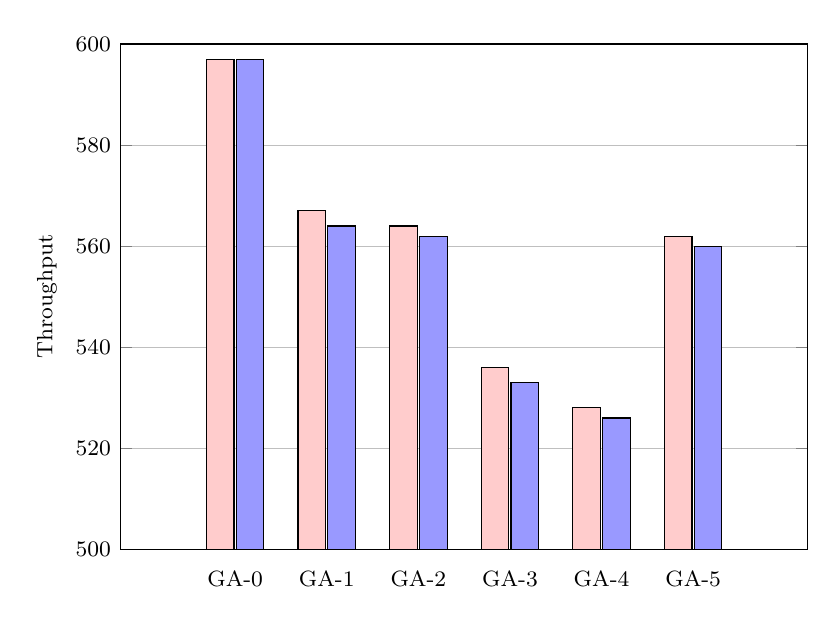
\begin{tikzpicture}[font=\footnotesize,baseline]
		\begin{axis}[
				width  = 0.85*\textwidth,
				height = 8cm,
				major x tick style = transparent,
				ybar=2*\pgflinewidth,
				bar width=10pt,
				ymajorgrids = true,
				ymin=500,
				ymax=600,
				ylabel = {Throughput},
				xticklabel={GA-\pgfmathprintnumber\tick},
				xtick = data,
				scaled y ticks = false,
				enlarge x limits=0.25,
				legend cell align=left,
				legend entries={$obj^*$: Scenario of optimization, $obj^{\textsc{SIM}}$: Scenario of simulation},
				legend to name=named,
				legend style={
					at={(10,6)},
					anchor=north east,
					column sep=1ex
				}
			]
			\addplot[color=black, fill=red!20,mark=none] coordinates {(0,597)(1,567)(2,564)(3,536)(4,528)(5,562)};
			\addplot[color=black,fill=blue!40,mark=none] coordinates {(0,597)(1,564)(2,562)(3,533)(4,526)(5,560)};
		\end{axis}
	\end{tikzpicture}
	\caption{Comparison of  Profile Results}

	\label{fig:88}
\end{figure}
			
					
\begin{longtable}{|c|c|c|c|c|c|c|c|c|r|}
    \hline
    & & \multicolumn{2}{c|}{Inputs} & \multicolumn{3}{c|}{Optimal assignment} & \multicolumn{2}{c|}{Worst assignment }& \\
    & \multicolumn{1}{c|}{ } & \multicolumn{1}{c|}{Profiles} & \multicolumn{1}{c|}{Mixprod}& \multicolumn{1}{c}{}   & \multicolumn{2}{c|}{} & \multicolumn{2}{c|}{}&\multicolumn{1}{c|}{}\\
    \it{GR} & \it{ID} & \multicolumn{1}{c|}{$(n_0,..,n_5)$} & \multicolumn{1}{c|}{$(I_1,..,I_3)$} & {$(a^*_1,..,a^*_6)$} & \it{obj}$^*$ & $(q^*_1$,...,$q^*_3)$ & {$(a^{\textsc{w}}_1,..,a^{\textsc{w}}_6)$} & \it{obj}$^{\textsc{w}}$ & \it{\%gap} \\ % [0.5ex]
    \hline
    & 7 & 5,1,0,0,0,0 & 1,0,0 & 1,0,0,0,0,0 & 597 & 597,0,0 & 0,1,0,0,0,0 & 567 & 5.0        \\
    & 8 & 5,0,1,0,0,0 & 1,0,0 & 2,0,0,0,0,0 & 597 & 597,0,0 & 0,2,0,0,0,0 & 564 & 5.5        \\
 GB & 9 & 5,0,0,1,0,0 & 1,0,0 & 0,0,0,0,3,0 & 597 & 597,0,0 & 0,3,0,0,0,0 & 536 & 10.2       \\
    & 10& 5,0,0,0,1,0 & 1,0,0 & 0,0,0,0,4,0 & 597 & 597,0,0 & 0,4,0,0,0,0 & 528 & 11.6       \\
    & 11& 5,0,0,0,0,1 & 1,0,0 & 0,0,0,0,5,0 & 597 & 597,0,0 & 0,5,0,0,0,0 & 562 & 5.9        \\
    \hline
    \caption{Results of Group B mixed scenarios} 													
    \label{tab:tr_gb}
\end{longtable}
										
Table~\ref{tab:tr_gb} presents the results of the scenarios considered in Group B (GB), which are comparable to the mixed scenario in the simulation section (in Table~\ref{tab:t0} -id $\in \{7..12\}$- from M11 to M16). The optimization process provides the optimal assignments of workers with non-perfect profiles, which ensures efficient use of resources and high-quality results.
			
All proposed solutions achieve optimal results when the perfect profile is assigned to the bottleneck machines (Machine 2 and Machine 4). The worst assignment occurs when the non-perfect profile is assigned to the first bottleneck machine (Machine 2). Similar results can be obtained by assigning the non-perfect profile to the second bottleneck machine (Machine 4). This confirms the classification obtained from the experimentation in group A (see Table~\ref{tab:tr_ga}).
    \begin{figure}[H]
	\centering
	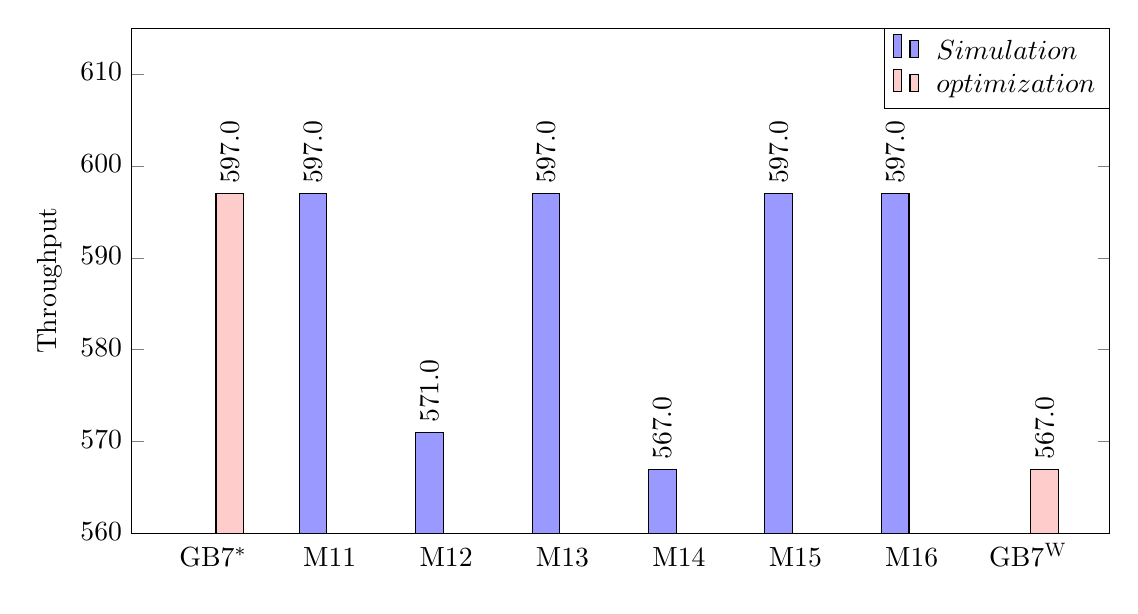
\begin{tikzpicture}
		\begin{axis}[
		      ybar,
				width=14cm,
				height=8cm,
				ymin=560,
				ymax=615,
				ylabel={Throughput},
				xtick=data,
			xticklabels={GB7$^{*}$,	M11, M12, M13, M14,	M15, M16, GB7$^{\textsc{W}}$},
				typeset ticklabels with strut,
				major tick length=0pt,
				major y tick style={/pgfplots/major tick length=1.5mm},
				nodes near coords always on top/.style={
				scatter/position=absolute,
				positive value/.style={
	   			at={(axis cs:\pgfkeysvalueof{/data point/x},\pgfkeysvalueof{/data point/y})},
				},
				negative value/.style={
				    at={(axis cs:\pgfkeysvalueof{/data point/x},0)},
				},
				every node near coord/.append style={
				    check values/.code={%
					\begingroup
					    \pgfkeys{/pgf/fpu}%
						\pgfmathparse{\pgfplotspointmeta<0}%
									\global\let\result=\pgfmathresult
									\endgroup
									\pgfmathfloatcreate{1}{1.0}{0}%
									\let\ONE=\pgfmathresult
									\ifx\result\ONE
										\pgfkeysalso{/pgfplots/negative value}%
									\else
										\pgfkeysalso{/pgfplots/positive value}%
									\fi
								},
								check values,
								anchor=west,
								rotate=90,
							},
						},
						nodes near coords={
							\pgfmathprintnumber[fixed zerofill,precision=1]{\pgfplotspointmeta}
						},
						nodes near coords always on top,
      	                legend cell align=left,
						legend entries={$Simulation$,$optimization$},
						legend style={
							at={(1,1)},
							anchor=north east,
							column sep=1ex
						}
					]
						
					\addplot [draw=black,fill=blue!40] coordinates {(0,0)  (1,597) (2,571)  (3,597)  (4,567) (5,597) (6,597)   (7,0)}; 
																												   
					\addplot [draw=black,fill=red!20] coordinates {(0,597) (7,567)}; 
																												   
				\end{axis}
			\end{tikzpicture}
   \caption{Scenario Simulations Mixed k=1 VS Scenario optimization id =7}
			\label{fig:mk1}
		\end{figure}
	
To compare optimization results with simulation (Figure~\ref{fig:mk1})  ones for mixed scenarios, we analyzed, for example, scenario 7 in Table~\ref{tab:tr_gb} to simulations (M11 to M16) (c.f. Table~\ref{tab:t0}) with $k=1$. Simulation results ranged between worst and best optimization solutions, confirming the reliability of optimization across all scenarios.
	
	
\begin{longtable}{|c|c|c|c|c|c|c|c|c|r|}
	\hline
	& & \multicolumn{2}{c|}{Inputs} & \multicolumn{3}{c|}{Optimal assignment} & \multicolumn{2}{c|}{Worst assignment }& \\
	& \multicolumn{1}{c|}{ } & \multicolumn{1}{c|}{Profiles} & \multicolumn{1}{c|}{Mixprod}& \multicolumn{1}{c}{}  & \multicolumn{2}{c|}{} & \multicolumn{2}{c|}{}&\multicolumn{1}{c|}{}\\
	\it{GR} & \it{ID} & \multicolumn{1}{c|}{$(n_0,..,n_5)$} & \multicolumn{1}{c|}{$(i_1,i_2,i_3)$} & {$(a^*_1,..,a^*_6)$} & \it{obj}$^*$ & $(q^*_1$,...,$q^*_3)$ & {$(a^{\textsc{w}}_1,..,a^{\textsc{w}}_6)$} & \it{obj}$^{\textsc{w}}$ & \it{\%gap} \\ % [0.5ex]
																										
																
	\hline
	        & 12      & 4,2,0,0,0,0                         & 1,0,0                                & 1,0,0,0,1,0          & 597          & 597,0,0               & 0,1,0,1,0,0                                & 567                     & 5.0        \\
	        & 13      & 4,0,2,0,0,0                         & 1,0,0                                & 2,0,0,0,2,0          & 597          & 597,0,0               & 0,2,0,2,0,0                                & 564                     & 5.5        \\
	GC      & 14      & 4,0,0,2,0,0                         & 1,0,0                                & 3,0,0,0,3,0          & 597          & 597,0,0               & 0,3,0,3,0,0                                & 536                     & 10.2       \\
	        & 15      & 4,0,0,0,2,0                         & 1,0,0                                & 4,0,0,0,4,0          & 597          & 597,0,0               & 0,4,0,4,0,0                                & 528                     & 11.5       \\
	        & 16      & 4,0,0,0,0,2                         & 1,0,0                                & 5,0,0,0,0,5          & 597          & 597,0,0               & 0,5,0,5,0,0                                & 562                     & 5.8        \\
	\hline
	        & 17      & 3,3,0,0,0,0                         & 1,0,0                                & 1,0,0,0,1,1          & 597          & 597,0,0               & 0,1,1,1,0,0                                & 567                     & 5.0        \\
	        & 18      & 3,0,3,0,0,0                         & 1,0,0                                & 2,0,0,0,2,2          & 597          & 597,0,0               & 0,2,2,2,0,0                                & 564                     & 5.5        \\
	GD      & 19      & 3,0,0,3,0,0                         & 1,0,0                                & 3,0,0,0,3,3          & 597          & 597,0,0               & 0,3,3,3,0,0                                & 536                     & 10.2       \\
	        & 20      & 3,0,0,0,3,0                         & 1,0,0                                & 4,0,4,0,4,0          & 597          & 597,0,0               & 0,4,4,4,0,0                                & 528                     & 11.5       \\
	        & 21      & 3,0,0,0,0,3                         & 1,0,0                                & 5,0,0,0,5,5          & 597          & 597,0,0               & 0,5,5,5,0,0                                & 562                     & 5.8        \\
	\hline
	        & 22      & 2,4,0,0,0,0                         & 1,0,0                                & 1,0,1,0,1,1          & 596          & 596,0,0               & 0,1,1,1,0,1                                & 567                     & 4.8        \\
	        & 23      & 2,0,4,0,0,0                         & 1,0,0                                & 2,0,2,0,2,2          & 596          & 596,0,0               & 0,2,2,2,0,2                                & 564                     & 5.3        \\
	GE      & 24      & 2,0,0,4,0,0                         & 1,0,0                                & 3,0,3,0,3,3          & 596          & 596,0,0               & 0,3,3,3,0,3                                & 536                     & 10.0       \\
	        & 25      & 2,0,0,0,4,0                         & 1,0,0                                & 4,0,4,0,4,4          & 596          & 596,0,0               & 0,4,4,4,0,4                                & 528                     & 11.4       \\
	        & 26      & 2,0,0,0,0,4                         & 1,0,0                                & 5,0,5,0,5,5          & 596          & 596,0,0               & 0,5,5,5,0,5                                & 562                     & 5.7        \\
	\hline
	        & 27      & 1,5,0,0,0,0                         & 1,0,0                                & 1,0,1,1,1,1          & 567          & 567,0,0               & 1,1,1,1,0,1                                & 567                     & 0.0        \\
	        & 28      & 1,0,5,0,0,0                         & 1,0,0                                & 2,0,2,2,2,2          & 564          & 564,0,0               & 2,2,2,2,0,2                                & 564                     & 0.0        \\
	GF      & 29      & 1,0,0,5,0,0                         & 1,0,0                                & 3,0,3,3,3,3          & 536          & 536,0,0               & 3,3,3,3,0,3                                & 536                     & 0.0        \\
	        & 30      & 1,0,0,0,5,0                         & 1,0,0                                & 4,4,4,0,4,4          & 528          & 528,0,0               & 4,4,4,4,0,4                                & 528                     & 0.0        \\
	        & 31      & 1,0,0,0,0,5                         & 1,0,0                                & 5,5,5,0,5,5          & 562          & 562,0,0               & 5,5,5,5,0,5                                & 562                     & 0.0        \\
	\hline
	\caption{Results of the GC, FD, GE, and GF scenario groups} 				
	\label{tab:tr_gcdef}
\end{longtable}
					
When comparing Table \ref{tab:tr_ga}, Table \ref{tab:tr_gb}, and Table \ref{tab:tr_gcdef}, it can be inferred that the scenarios of the GC, GD, GE, and GF scenario groups fall between the GB scenario (minimum) and the GA scenario (maximum), in terms of the impact of each profile on throughput.
The observation of the gap in each group correlates with the ranking of profiles deduced from the results of scenarios GA. In fact, we obtain each time the most important gap with scenarios 10,15, 20, and 25 where profile 5 is selected. By the same reasoning, the lowest gap is obtained by selecting profile number 1, as can be observed in Table~\ref{tab:tr_gb} and Table~\ref{tab:tr_gcdef}.    
			
The gap decreases when there are more workers with the same profile due to the degradation of the optimal assignment. For instance, when the number of workers with the fourth profile $n_4$ increases from 1 to 6 in scenarios 10, 15, 20, 25, 30, and 5, the corresponding gaps are 11.6, 11.5, 11.5, 11.4,0, and 0, respectively.
We can also observe that the optimal solution for scenarios with more than two perfect profiles can reach the maximum throughput value because the number of perfect profiles is greater than or equal to the number of bottleneck machines. In the case of product of type 1 there are two bottleneck machines ($WS_2$ and $WS_4$), which are manipulated by a perfect profile in scenarios of groups GC, GD, GE, and GB. In scenarios GF and GA the is only one perfect profile which is not enough to each the maximum throughput (597). In the scenarios of group GF and GA the worst and the bast scenarios are providing the same throughput because the optimal worker allocation cannot avoid the effect of the non-perfect profile and provide the worst throughput of the other groups.
	
\begin{longtable}{|c|c|c|c|c|c|c|c|c|r|}
	\hline
	& & \multicolumn{2}{c|}{Inputs} & \multicolumn{3}{c|}{Optimal assignment} & \multicolumn{2}{c|}{Worst assignment }& \\
	& \multicolumn{1}{c|}{ } & \multicolumn{1}{c|}{Profiles} & \multicolumn{1}{c|}{Mixprod}& \multicolumn{1}{c}{}  & \multicolumn{2}{c|}{} & \multicolumn{2}{c|}{}&\multicolumn{1}{c|}{}\\
	& ID & \multicolumn{1}{c|}{$(n_0,..,n_5)$} & \multicolumn{1}{c|}{$(I_1,..,I_3)$} & {$(a^*_1,..,a^*_6)$} & \it{obj}$^*$ & $(q^*_1$,...,$q^*_3)$ & {$(a^{\textsc{w}}_1,..,a^{\textsc{w}}_6)$} & \it{obj}$^{\textsc{w}}$ & \it{\%gap}     \\ % [0.5ex]
	\hline
	& 32 & 0,1,1,1,1,2 & 1,0,0 &5,2,3,1,5,4 & 564 & 564,0,0 & 2,4,5,3,1,5 & 528 & 6.3\\
	& 33 & 0,2,2,1,1,0 & 1,0,0 &4,1,2,1,3,2 & 567 & 567,0,0 & 1,4,2,3,1,2 & 528 & 6.8\\
	& 34 & 1,1,0,3,0,1 & 1,0,0 &3,0,5,1,3,3 & 567 & 567,0,0 & 1,3,3,3,0,5 & 536 & 5.4\\
	  & 35 & 1,0,0,3,1,1 & 1,0,0 & 3,5,3,0,4,3 & 562 & 562,0,0 & 5,4,3,3,0,3 & 528 & 6.0 \\ & 
	36 & 0,3,0,0,3,0 & 1,0,0 &4,1,1,1,4,4 & 567 & 567,0,0 & 1,4,4,4,1,1 & 528 & 6.8\\
	& 37 & 1,1,1,1,0,2 & 1,0,0 &3,1,5,0,2,5 & 567 & 567,0,0 & 1,3,5,5,0,2 & 536 & 5.4\\
	& 38 & 0,0,4,2,0,0 & 1,0,0 &3,2,2,2,2,3 & 564 & 564,0,0 & 2,3,2,3,2,2 & 536 & 4.9\\
	& 39 & 2,3,0,1,0,0 & 1,0,0 &3,0,1,0,1,1 & 596 & 596,0,0 & 0,3,1,1,0,1 & 536 & 10.0\\
	& 40 & 0,5,0,0,1,0 & 1,0,0 &4,1,1,1,1,1 & 567 & 567,0,0 & 1,4,1,1,1,1 & 528 & 6.8\\
	& 41 & 1,0,5,0,0,0 & 1,0,0 &2,0,2,2,2,2 & 564 & 564,0,0 & 2,2,2,2,0,2 & 564 & 0.0\\
	& 42 & 0,0,3,1,2,0 & 1,0,0 &3,2,4,2,4,2 & 564 & 564,0,0 & 2,4,3,4,2,2 & 528 & 6.3\\
	& 43 & 1,0,4,0,1,0 & 1,0,0 &2,0,2,2,4,2 & 564 & 564,0,0 & 2,4,2,2,0,2 & 528 & 6.3\\
	{GG}\label{SEN:GG} & 44 & 0,1,0,5,0,0 & 1,0,0 &3,3,3,1,3,3 & 536 & 536,0,0 & 3,3,3,3,1,3 & 536 & 0.0\\
	& 45 & 0,1,2,0,2,1 & 1,0,0 &2,2,5,1,4,4 & 564 & 564,0,0 & 2,4,5,4,1,2 & 528 & 6.3\\
	& 46 & 0,0,3,0,3,0 & 1,0,0 &2,2,4,2,4,4 & 564 & 564,0,0 & 2,4,4,4,2,2 & 528 & 6.3\\
	& 47 & 1,4,0,0,1,0 & 1,0,0 &1,0,1,1,1,4 & 567 & 567,0,0 & 1,4,1,1,0,1 & 528 & 6.8\\
	& 48 & 0,3,0,1,1,1 & 1,0,0 &3,1,5,1,1,4 & 567 & 567,0,0 & 1,4,5,3,1,1 & 528 & 6.8\\
	& 49 & 0,0,3,2,1,0 & 1,0,0 &3,2,4,2,2,3 & 564 & 564,0,0 & 2,4,3,3,2,2 & 528 & 6.3\\
	& 50 & 0,5,0,0,1,0 & 1,0,0 &4,1,1,1,1,1 & 567 & 567,0,0 & 1,4,1,1,1,1 & 528 & 6.8\\
	& 51 & 3,1,0,2,0,0 & 1,0,0 &3,0,1,0,3,0 & 597 & 597,0,0 & 0,3,1,3,0,0 & 536 & 10.2\\
	& 52 & 1,2,0,2,1,0 & 1,0,0 &3,0,1,1,3,4 & 567 & 567,0,0 & 1,4,3,3,0,1 & 528 & 6.8\\
	& 53 & 0,1,1,0,4,0 & 1,0,0 &1,4,4,2,4,4 & 564 & 564,0,0 & 2,4,4,4,1,4 & 528 & 6.3\\
	& 54 & 2,0,1,0,1,2 & 1,0,0 &4,0,2,0,5,5 & 596 & 596,0,0 & 0,4,5,5,0,2 & 528 & 11.4\\
	& 55 & 0,0,2,0,4,0 & 1,0,0 &4,2,4,2,4,4 & 564 & 564,0,0 & 2,4,4,4,2,4 & 528 & 6.3\\
	\hline
	\hline
	\caption{Results of the GG scenario group} 
	\label{tab:tr_gg}
\end{longtable}
					
Table~\ref{tab:tr_gg} presents the results of various scenarios that take into account a mix of profiles. It should be noted that only the scenario with more than two perfect profiles is able to achieve the maximum throughput of 597, which confirms our previous observation in Table~\ref{tab:tr_gb}. The optimal allocation strategy involves assigning the best available profiles to the bottleneck workstation with the longest processing time. We also observe that the largest gaps between the best and worst allocation strategies are obtained when multiple perfect profiles are available, owing to the high throughput of the optimal solution. Conversely, the presence of several similar profiles tends to reduce the gap between the best and worst allocation strategies, as evidenced by scenarios 41 and 44. These findings provide valuable insights for optimizing resource allocation and improve overall system performance in manufacturing environments.
					
The results obtained clearly demonstrate the significant impact of operator behaviour on the productivity of a production system, even if it is a relatively straightforward system producing a single type of product in a flow shop configuration. The findings underscore the importance of recognizing the role of human factors in manufacturing processes and highlight the need for targeted interventions to optimize performance. These insights have broader implications for enhancing productivity and efficiency in a variety of industrial settings.
				   
					
					
\begin{longtable}{|c|c|c|c|c|c|c|c|c|r|}
	\hline
	& & \multicolumn{2}{c|}{Inputs} & \multicolumn{3}{c|}{Optimal assignment} & \multicolumn{2}{c|}{Worst assignment }& \\
	& \multicolumn{1}{c|}{ } & \multicolumn{1}{c|}{Profiles} & \multicolumn{1}{c|}{Mixprod}& \multicolumn{1}{c}{}  & \multicolumn{2}{c|}{} & \multicolumn{2}{c|}{}&\multicolumn{1}{c|}{}\\
	\it{GR}            & \it{ID} & \multicolumn{1}{c|}{$(n_0,..,n_5)$} & \multicolumn{1}{c|}{$(I_1,..,I_3)$} & {$(a^*_1,..,a^*_6)$} & \it{obj}$^*$ & $(q^*_1$,...,$q^*_3)$ & {$(a^{\textsc{w}}_1,..,a^{\textsc{w}}_6)$} & \it{obj}$^{\textsc{w}}$ & \it{\%gap} \\ % [0.5ex]
									
	\hline 
									
	                   & 56      & 1,1,1,1,1,1                         & 1,0,0                               & 4,2,3,0,1,5          & 112          & 112,0,0               & 1,4,5,3,0,2                                & 103                     & 8.0        \\
	                   & 57      & 1,1,1,1,1,1                         & 0,1,0                               & 1,0,3,4,2,5          & 118          & 0,118,0               & 1,4,5,3,0,2                                & 112                     & 5.0        \\
	                   & 58      & 1,1,1,1,1,1                         & 0,0,1                               & 3,0,5,2,4,1          & 138          & 0,0,138               & 1,4,5,3,0,2                                & 136                     & 1.4        \\
	{GH}\label{SEN:GH} & 59      & 1,1,1,1,1,1                         & 1,1,0                               & 4,0,3,2,1,5          & 121          & 5,116,0               & 1,4,5,3,0,2                                & 115                     & 4.9        \\
	                   & 60      & 1,1,1,1,1,1                         & 1,0,1                               & 4,0,3,1,2,5          & 138          & 1,0,137               & 1,4,5,3,0,2                                & 136                     & 1.4        \\
	                   & 61      & 1,1,1,1,1,1                         & 0,1,1                               & 3,0,4,2,5,1          & 142          & 0,35,107              & 1,4,5,3,0,2                                & 139                     & 2.1        \\
	                   & 62      & 1,1,1,1,1,1                         & 1,1,1                               & 1,4,3,0,2,5          & 147          & 7,18,122              & 1,4,5,3,0,2                                & 141                     & 4.0        \\
									
									        
	\hline
	\caption{Results of the GH scenario group} 
	\label{tab:tr4}
\end{longtable}
			
					

				
The aim of the last scenario group (GH) is to test the efficiency of the proposed model when several product types are considered. In this situation, the optimization model will determine the best assignment of workers,  the amount of production for each product type, and the scheduling of all product operations in order to Maximize production throughput. Due to the complexity of the problem, we reduced the optimization horizon from one week to one day. We also considered several product mixes (ProdMix), as shown in Table~\ref{tab:tr4}. We notice that Mixprod has a significant impact on optimal assignment and productivity. 
			
After analysing scenarios 56, 57, and 58, it is clear that selecting type 3 of the product leads to the highest throughput. This is mainly due to its better workstation balancing, which results in a shorter cycle time of only 3 time units. Although type 3 has the longest total processing time of 16 time units, it more than compensates for it with its other advantages, making it the optimal choice to achieve maximum throughput.  
		
Scenarios 59, 60 and 61 propose the production of two types of products with minimal production (production mix) of one part $q_t^{min}= 1$. When comparing scenario 59 (selection of product types 1 and 2) with scenarios 56 (product type 1) and 57 (product type 2), it is clear that the productivity of scenario 59 has been improved due to the scheduling of jobs by product type. However, the optimal solution generates 5 products of type 1 and 116 of product type 2 due to the reduced total processing time of the type 2 product (15 time unit for type 1 VS 11 time unit for type 2) and the same nominal cycle time of 4 time units. 
			
			
In Scenario 60, we observe that the optimal solution involves producing 137 units of type 3 and only one unit of type 1. Conversely, scenario 58 revealed that the optimal solution includes 138 units of type 1. This indicates that the production of type 1 product is not ideal for maximising throughput and is instead only necessary due to the constraint outlined in (\ref{c7}), which requires the production of at least one unit of type 1 product to be produced.
The maximum throughput corresponds to the scenario 62 (with an optimal throughput of 147) where all types of product are selected. This allows to conclude that the productivity increases as we have a large number of product types. 
The optimal assignment of the worker profile tray to increase the balance of the production line based on the punctuality of profiles. For example, in the scenario 56 that the best profiles are assigned to the worst machines, which increases the balancing of the lines and increases the production system throughput. 
	
						       
					
\section{Managerial insights }\label{sec:mins}
This study emphasises the critical role of effective human resource allocation strategies in achieving maximum throughput in manufacturing environments. Assignment of the best worker profiles to bottleneck workstations is particularly crucial for success. The largest gaps between the best and worst allocation strategies are observed when multiple perfect profiles are available, highlighting the importance of such strategies. The problem becomes more complex when it is not easy to define the bottleneck machine due to the production of different types of products with different processing times.  
The study also underscores the significant impact of operator behaviour on productivity in a production system, highlighting the need to recognise human factors and implement targeted interventions for optimal performance. These insights can help improve productivity and efficiency in various industrial settings. Additionally, the study demonstrates that the selection of the right product type is essential to optimize the efficiency of an optimization model to Maximize production throughput. Choosing the product with the smallest nominal cycle time resulted in the highest throughput, despite having a longer total processing time, due to better balancing of the workstation. Furthermore, a larger number of product types can increase productivity, and optimizing the assignment of worker profiles can improve line balancing and further increase production system throughput. Finally, the study highlights the importance of selecting mixed team workers, particularly in manufacturing systems with a high mix of production. While the manager may not be able to determine the exact dynamic effect of one worker on another, assigning a specific worker with particular behavior will still influence the assignment of other workers, whether they have equivalent or different behavior and skills. 
% \textcolor{red}{  --- worker team importance. }
			
					
\section{Conclusions and future works  }\label{sec:conc3}  
This work presents an approach for modelling, simulating, and optimizing the impact of human behaviour on production throughput. A stochastic approach to model human behaviour in terms of punctuality on the workstation is proposed and simulated in a dual resource flow-shop production system. A non-linear optimization model is proposed to provide the optimal assignment of workers to machines, the optimal scheduling of production operations, and the optimal mix of production to maximize production throughput, while considering the possibility of operations interruption. The results show that human behaviour has an important influence on the productivity of the production system, especially when the number of product and worker profiles increases. The analyses of results demonstrate the complexity of selecting the best worker profile for the best machine, especially in high-mix production systems. In flow shop production systems, it is very important to ensure a good balance of the production line, and the assignment of human workers plays an important role in maximising the throughput of the production system.  
	
In the next step, we plan to improve our human behaviour models by incorporating factors such as experience, skills, and personality to improve the accuracy of the proposed optimization model.
Moreover, it will be worthwhile to develop approximate methods (e.g. metaheuristics) to solve the proposed optimization model in order to be able to handle more realistic cases in terms of instance size.
Another interesting perspective of this work involves the evolution of behavior through the improvement of skill levels and the impact of one worker on another within the same team.
% \textcolor{red}{   talking about the consideration of the interaction between operators in a single team. }
To validate our theoretical results, we will to apply our approach to a real-world case study and observe the impact of optimal worker behaviour on system performance in a dynamic environment. This will not only help validate our approach, but also provide valuable data for predicting worker states and integrating that information into an adaptive decision-making process for worker assignment and production task scheduling. Our ultimate goal is to develop a robust and effective optimization model that considers the human factor in manufacturing processes to improve productivity and efficiency while also improving human well-being in a manufacturing environment.
	
%\section*{Acknowledgment}\label{sec:Acknow}
%Acknowledgement is made to the Normandy region and the European Union for supporting this research through the RIN regional research programme by funding the AntiHpert project.

%% If you have bibdatabase file and want bibtex to generate the
%% bibitems, please use
%%
% \listoffigures
% \listoftables
%\newpage
\thispagestyle{empty}
 \bibliographystyle{elsarticle-num} 
 
 
 \bibliography{cas-refs2}


%% else use the following coding to input the bibitems directly in the
%% TeX file.

% \begin{thebibliography}{00}

% %% \bibitem{label}
% %% Text of bibliographic item

% \bibitem{}

% \end{thebibliography}
\end{document}
\endinput
%%
%% End of file `elsarticle-template-num.tex'.
